\documentclass{cshonours}

\usepackage{graphics}  % For figures
\usepackage{amsmath}   % For mathematical expressions
\usepackage{amssymb}   % For mathematical symbols
\usepackage{booktabs}  % For professional tables
\usepackage{array}     % For advanced column formatting
\usepackage{tabularx}  % For tables of a specific width
\usepackage{threeparttable} % For tables with notes
\usepackage{adjustbox} % To adjust box content (e.g., scale table)
\usepackage{makecell}  % For multi-line cells
\usepackage{subcaption}


\newcolumntype{L}{>{\raggedright\arraybackslash}X}
\newcolumntype{C}[1]{>{\centering\arraybackslash}p{#1}}

\title{Temporal Geometric Neural Networks for Rumour Detection: Architectures, Applications, and Temporal Nuance}
\author{[Matthew Haskins]} % Replace with your name

\keywords{Graph Neural Networks, Temporal Graph Neural Networks, Graph Attention Network, Dynamic Graphs, Rumour Detection, Social Network Analysis, Misinformation, Temporal Attention, PHEME Dataset}
\categories{I.2.6, H.2.8} % Computing methodologies - AI and Database applications - Data mining

\begin{document}
\maketitle

\begin{abstract}

\emph{Rumour detection} on social media hinges on recognising \emph{how} information propagates, not merely \emph{what} is said. To probe the role of temporal dynamics, we benchmark six graph-based neural models on the \emph{PHEME} Twitter corpus: static \emph{GCN}, \emph{GAT}, \emph{GATv2}, and three dynamic variants—\emph{DySAT}, a \emph{simplified DySAT} without temporal self-attention, and the continuous-time \emph{Temporal Graph Network} (TGN). Results show that temporal self-attention is valuable but not transformative: full DySAT edges out its aggregation-only ablation by roughly 3 percentage points in macro-F1, confirming that fine-grained time weighting helps but that much of the signal is already captured by simpler temporal aggregation. By contrast, TGN fails to surpass even our static graph baseline, suggesting that its memory-update mechanism is ill-suited to PHEME’s sparse, subtle temporal cues. Among static methods, \emph{GATv2} delivers a consistent yet modest improvement over GAT, illustrating the benefit of more expressive attention even without explicit temporal modelling. Qualitative assessments of t-SNE projections further reveal that temporal models carve cleaner rumour/non-rumour clusters than static ones, underscoring a geometric advantage. Collectively, these findings indicate that effective rumour detection benefits from architectures that embed temporal reasoning directly, while also cautioning that not all continuous-time designs transfer cleanly to real-world social datasets. 

\end{abstract}


\tableofcontents
\listoffigures

\chapter{Introduction}

False or unverified claims now surge through social media with unprecedented speed and reach, shaping public opinion and even real-world behaviour~\cite{vosoughi2018spread}.  Twitter conversation threads, in particular, unfold as intricate cascades of replies and retweets whose topology and timing encode valuable clues about credibility.  The \emph{PHEME} corpus captures this phenomenon across major breaking-news events, providing thread-level labels that distinguish rumours from non-rumours~\cite{zubiaga2016pheme}.  Yet despite a decade of progress, automatic rumour detection remains challenging because it must parse both the \emph{content} of posts and the \emph{dynamics} of their propagation.


Graph Neural Networks (GNNs) offer a principled way to exploit the relational context of social conversations, propagating information along reply or retweet links so that each node embedding reflects its neighbourhood \cite{kipf2017semi}.  Early static models such as GCN and Bi-GCN already outperform text-only baselines on PHEME by modelling conversation structure \cite{bian2020rumor}, while attention-based variants (GAT) capture heterogeneous neighbour importance \cite{lv2022rumor}.  However, these approaches compress a dynamic process into a single snapshot, discarding temporal patterns that differentiate false from factual narratives—patterns documented at scale by Vosoughi and colleagues \cite{vosoughi2018spread} and echoed across subsequent misinformation studies \cite{survey2024disinfo}.


To reincorporate time, researchers have proposed two main paradigms.  \emph{Snapshot-based self-attention}, exemplified by \emph{DySAT}, learns joint structural–temporal attention over a sequence of graph slices, enabling nodes to weigh past states adaptively \cite{sankar2020dysat}.  At the other extreme, \emph{continuous-time memory} models such as the \emph{Temporal Graph Network} (TGN) update per-node memories at every interaction event, supporting fine-grained streaming inference \cite{rossi2020tgn}.  More recently, \emph{GATv2} extends static attention with query-dependent weights, narrowing the expressiveness gap between time-agnostic and time-aware designs \cite{brody2022gatv2}.


Although temporal mechanisms are intuitively appealing, their real-world benefit is still an open question.  The literature reports substantial gains for DySAT on link-prediction benchmarks \cite{sankar2020dysat} and for TGN on interaction forecasting \cite{rossi2020tgn}, yet evidence from rumour detection is limited and sometimes contradictory \cite{liu2025rumor}.  Moreover, the additional complexity—larger hyper-parameter spaces, heavier computation, and harder interpretability—may not justify modest accuracy improvements \cite{survey2024disinfo}.  A systematic comparison on a common benchmark is therefore needed.


Leveraging the modular \emph{Araneos} platform, developed during the course of this research, we perform the first head-to-head evaluation of six representative architectures—GCN, GAT, GATv2, DySAT, a simplified DySAT without temporal attention, and TGN—on identical PHEME conversation graphs.  This design isolates the impact of temporal mechanisms embedded in model structure rather than in handcrafted features or data splits.  The investigation is guided by three questions:

\begin{enumerate}
    \item \emph{RQ1:} Do temporal GNNs achieve materially better rumour-detection performance than strong static counterparts on PHEME?  
    \item \emph{RQ2:} How much improvement, if any, does DySAT’s temporal self-attention deliver relative to simple temporal aggregation?  
    \item \emph{RQ3:} Why might a continuous-time memory model like TGN fail to outperform static baselines despite its success on other dynamic-graph tasks?  
\end{enumerate}


Addressing these questions advances both theory and practice.  Theoretically, it clarifies whether temporal reasoning should be baked into the \emph{architecture} of rumour-detection systems or can be emulated with richer static features and expressive attention \cite{choi2021dynGCN}.  Practically, it informs platform engineers who must balance detection accuracy against computational cost and interpretability—critical factors for real-time moderation pipelines \cite{survey2024disinfo}.  By exposing the conditions under which temporal dynamics help or hinder, this work charts a more evidence-based path toward trustworthy, scalable misinformation defences.


\chapter{Background}\label{chap:background}

Rumour detection occupies a nexus of natural-language understanding, network science, and temporal data analysis.  A single Twitter thread weaves together user roles, linguistic stance, and the high-velocity cascade by which information fans out across the platform.  Over roughly ten years, the research community has pursued this multilayered signal through five overlapping neural “eras.”  Each era offered a sharper lens but also revealed fresh blind spots, ultimately pointing toward Temporal Graph Neural Networks (TGNNs)—the architectural family whose strengths and open questions motivate the experiments in this thesis.  This chapter retraces that trajectory, formalises core graph-learning concepts for readers versed in mainstream deep learning, and establishes the conceptual bridge to the dedicated literature review that follows.  

Figure \ref{fig:timeline} summarises the milestones, while Figure \ref{fig:temporal_overview} previews how temporal GNNs extend static message passing.

%%%%%%%%%%%%%%%%%%%%%%%%%%%%%%%%%%%%%%%%%%%%%%%%%%%%%%%%%%%%%%%%
\begin{figure}[htbp]
  \centering
  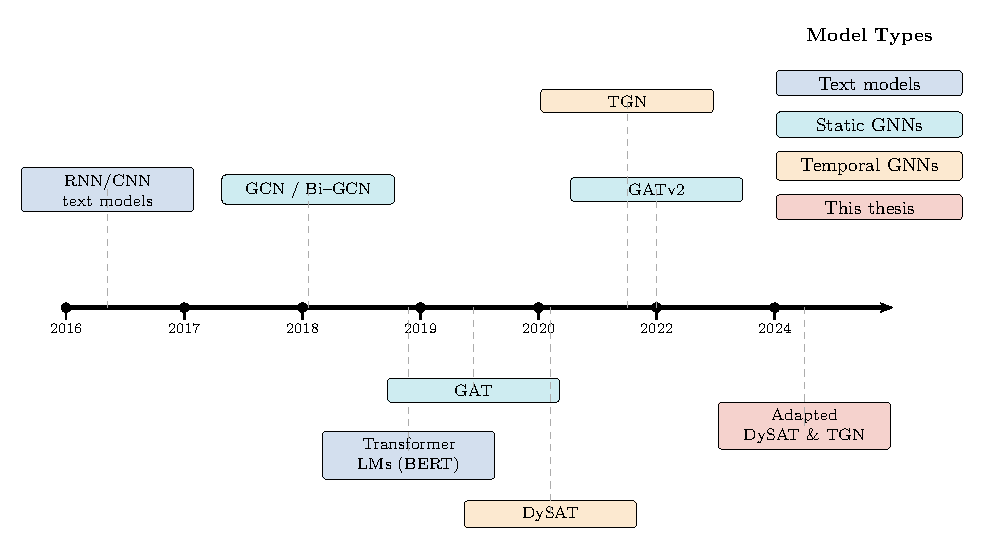
\includegraphics[width=\textwidth]{../figures/rumour_timeline.pdf}
  \caption{Evolution of neural approaches to rumour detection.  Text-sequence models led to contextual language models; propagation-aware hybrids introduced handcrafted graph cues; static Graph Neural Networks (GNNs) unified content and structure; Temporal GNNs embed timing directly in the learning process.}
  \label{fig:timeline}
\end{figure}
%%%%%%%%%%%%%%%%%%%%%%%%%%%%%%%%%%%%%%%%%%%%%%%%%%%%%%%%%%%%%%%%

\section{From Sequential to Structural Thinking}

Early neural systems framed rumour detection as a purely \emph{sequential} problem: RNNs and CNNs scanned token streams \cite{yu2017cnn}, and later Transformers further enlarged the lexical receptive-field \cite{rahman2024primer}. Yet these models implicitly flattened the social conversation—reply trees, user interactions, temporal retweets—into a one-dimensional string, forcing researchers to bolt on handcrafted graph features that only partially captured how misinformation diffuses. Because a rumour’s credibility often hinges on \emph{who} shares it, \emph{when}, and along \emph{which} relational paths, the research community pivoted toward a \emph{structural} view: Graph Neural Networks (GNNs) treat users as nodes, interactions as edges, and learn to pass messages along the very propagation channels that make rumours viral \cite{bian2020rumor}. This shift unifies textual semantics with network topology in a single differentiable framework, delivering better generalisation across events and platforms while eliminating brittle feature engineering. 
\section{Graph Neural Networks: A Unified Structural Lens}


Let a directed graph be \(G=(V,E)\) with \(|V|=N\) nodes and \(|E|\) edges.  Each node \(v\in V\) carries an initial feature vector \(\mathbf{x}_v\in\mathbb{R}^{d_0}\); edges may hold attributes \(\mathbf{e}_{uv}\).  In a social-media conversation, nodes can represent tweets, users, or both; edges encode reply, retweet, or mention relationships.  The adjacency matrix \(A\) (or sparse edge list) captures topology, while a timestamp \(t_{uv}\) records when edge \((u,v)\) occurred.


Most contemporary GNNs follow the Message-Passing Neural Network (MPNN) template.  For layer \(l\) and node \(i\),
\begin{equation}
\mathbf{h}_i^{(l+1)}
=\sigma\!\Bigl(
f_{\text{comb}}\!\bigl(
\mathbf{h}_i^{(l)},\;
f_{\text{agg}}\bigl\{
g_{\text{msg}}\!\bigl(
\mathbf{h}_i^{(l)},\mathbf{h}_j^{(l)},\mathbf{e}_{ij}\bigr)
\; : j\!\in\!\mathcal{N}(i)\bigr\}\bigr)
\Bigr),
\label{eq:mpnn}
\end{equation}
where  
\(g_{\text{msg}}\) maps an edge to a message,  
\(f_{\text{agg}}\) is permutation invariant (sum, mean, max, attention),  
\(f_{\text{comb}}\) fuses aggregated evidence with the node state,  
and \(\sigma\) is an activation \cite{gnn_applications_2024}.  
Stacking \(L\) layers yields embeddings that capture up-to-\(L\)-hop structural context.


The Graph Convolutional Network (GCN) instantiates Eq.~\eqref{eq:mpnn} by using  
\(g_{\text{msg}}(\mathbf{h}_j)=\mathbf{h}_j\),  
\(f_{\text{agg}}=\textstyle\sum\nolimits_{j}\tilde{D}^{-1/2}\tilde{A}_{ij}\tilde{D}^{-1/2}\mathbf{h}_j\),  
and \(f_{\text{comb}}(\cdot)=W^{(l)}(\cdot)\) \cite{kipf2017semi}.  
The symmetric normalisation \(\tilde{D}^{-1/2}\tilde{A}\tilde{D}^{-1/2}\) ensures each message is weighted by node degree, providing a spectral approximation of Laplacian smoothing.  In rumour detection, Bi-GCN extended this principle by separating top-down from bottom-up propagation along conversation trees, yielding state-of-the-art F\(_1\) above 0.89 on Twitter15/16 datasets and 0.802 on PHEME \cite{bian2020rumor}.


Graph Attention Networks (GAT) replace fixed degree weights with learned coefficients  
\(\alpha_{ij}=\text{softmax}_j\bigl(\text{LeakyReLU}(\mathbf{a}^\top[W\mathbf{h}_i\|\;W\mathbf{h}_j])\bigr)\),  
allowing each node to emphasise informative neighbours and dampen noise \cite{velickovic2018gat}.  GATv2 removes the static key–query ordering, granting full query-adaptive weights and provably higher expressiveness \cite{brody2022gatv2}.  In practice, attention heat-maps often highlight authoritative denials or sceptical users, offering interpretability absent from sequence models.


Despite unifying content and structure, static GNNs freeze time.  They cannot differentiate a rumour that explodes and dies within an hour from one diffusing slowly but reaching comparable breadth.  Empirically, spread velocity, burstiness, and correction latency strongly distinguish misinformation from factual news \cite{vosoughi2018spread}.  Further, deep message passing can \emph{over-squash} long-range signals into fixed-width embeddings, hampering reasoning across many hops \cite{oversquashing_gnn_2025}.  Finally, the representational power of standard MPNNs is bounded by the first-order Weisfeiler–Lehman test \cite{xu2019gin}, restricting discrimination of topologically similar yet temporally divergent cascades.


\section{Temporal Graph Neural Networks}


A \emph{temporal} or \emph{dynamic} graph augments \(E\) with a timestamp map  
\(\tau:E\!\to\!\mathbb{R}_{\ge0}\).  
Learning tasks can model discrete “snapshots” \(G_1,\dots,G_S\) sampled at interval \(\Delta t\) or continuous-time event streams where each edge arrives asynchronously.  Rumour cascades exhibit both coarse timeline stages (breaking, correction, decay) and fine-grained micro-interactions (reply chains firing within seconds), making temporal modelling attractive.


Recent surveys categorise TGNNs along two axes \cite{dynamic_gnn_survey_2024}:  

\begin{enumerate}
\item \emph{Snapshot-based} methods process an ordered sequence of graphs and often apply attention to weigh historical snapshots.  
\item \emph{Continuous-time} methods update node states upon each event via time-aware memories or point-process kernels.
\end{enumerate}

The remainder of this thesis evaluates representative architectures from both families—DySAT (snapshot self-attention) and TGN (continuous-time memory)—because they capture complementary inductive biases that may benefit rumour detection.

\paragraph{DySAT (snapshot self-attention).}
DySAT introduces dual self-attention:  
structural attention learns intra-snapshot importance, while temporal attention learns which historical snapshots matter when predicting node states \cite{sankar2020dysat}.  
This design captures both local neighbourhood influence and overarching temporal evolution.

\paragraph{TGN (continuous-time memory).}
Temporal Graph Networks associate each node with a recurrent memory.  
Upon receiving an event \((u,v,t)\), time-encoded messages update memories \(\mathbf{m}_u,\mathbf{m}_v\); a readout module then combines memory and static features to produce on-the-fly embeddings \cite{rossi2020tgn}.  
Such memory systems support millisecond-level resolution and naturally model irregular interaction gaps.


Rumour cascades exhibit temporal signatures such as rapid early diffusion, late mass corrections, or user-credibility shifts over time.  Snapshot attention can weigh such phases differently, while continuous-time memories can reflect recency effects (e.g.\ “fresh” corrections damp rumour credibility more than stale ones).  Evaluating both paradigms therefore illuminates whether temporal granularity or modelling mechanism drives performance on PHEME.

%%%%%%%%%%%%%%%%%%%%%%%%%%%%%%%%%%%%%%%%%%%%%%%%%%%%%%%%%%%%%%%%
\begin{figure}[htbp]
  \centering
  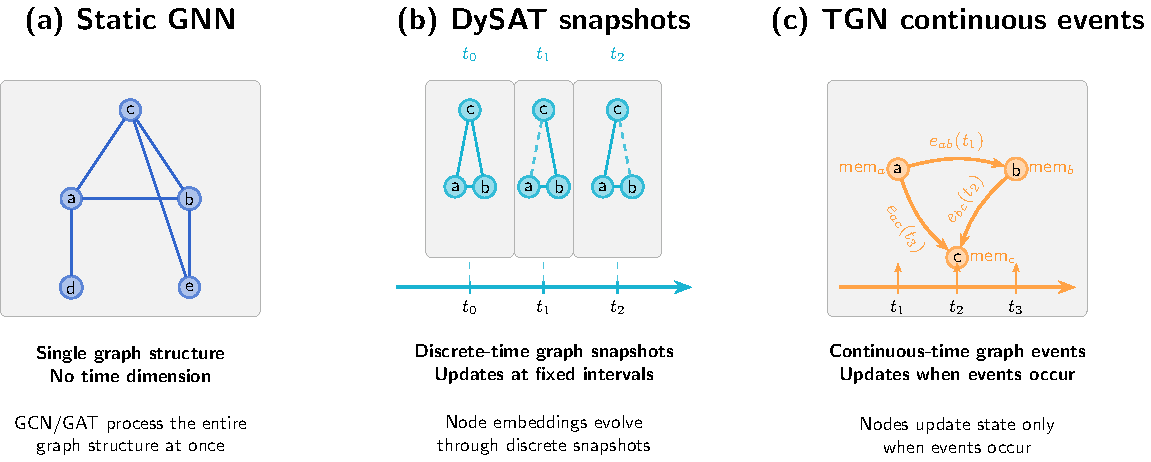
\includegraphics[width=.9\textwidth]{../figures/static_vs_temporal.pdf}
  \caption{Static vs.~temporal processing.  (a) Static GNN views a single aggregated graph. (b) DySAT applies structural \emph{and} temporal self-attention across ordered snapshots. (c) TGN streams individual events and updates node memories in continuous time.  Both paradigms aim to preserve timing cues lost in static aggregation.}
  \label{fig:temporal_overview}
\end{figure}
%%%%%%%%%%%%%%%%%%%%%%%%%%%%%%%%%%%%%%%%%%%%%%%%%%%%%%%%%%%%%%%%


The panorama above shows how each methodological generation sharpened the rumour-detection lens:  
text models decoded \emph{content}, hybrids injected handcrafted \emph{context}, static GNNs \emph{learned} context, and TGNNs finally weave \emph{time} into representation learning.  Yet questions remain: Which temporal paradigm works best for sparse, high-burst datasets such as PHEME?  Does temporal modelling truly outperform expressive static attention, or are gains confined to dense dynamic graphs?  The next chapter surveys specialised TGNN literature and positions those questions within current research frontiers.


\chapter{Literature Review}\label{chap:literature}

Building on the background trajectory, this chapter reviews prior approaches to rumour detection with a focus on how temporal dynamics have (or have not) been integrated. We first outline the literature search methodology, then synthesize related work in five thematic areas: early text-centric models, static graph-based models, emerging temporal GNN frameworks, prevailing evaluation practices, and considerations for interpretability and deployment. We conclude by identifying key gaps and tensions in the literature and linking them to our research questions.

\section{Search Strategy}
We conducted a comprehensive search of academic databases and repositories to capture relevant studies from 2015 through 2024. Keyword combinations targeting the domain and task were used, including variants of “rumour”/“rumor” paired with terms like “detection,” “propagation,” “graph neural network,” “dynamic graph,” and “temporal model.” We searched Google Scholar, the ACL Anthology, IEEE Xplore, and arXiv pre-print server to ensure coverage of both peer-reviewed publications and influential preprints. To ground the review in comparable benchmarks, we filtered for works evaluating on established rumour datasets such as \emph{PHEME}~\cite{zubiaga2016pheme} and the Twitter$_{15}$ and Twitter$_{16}$ tweet conversation sets introduced by Ma \textit{et al.}~\cite{ma2017rumordatasets}. We primarily included English-language papers from conferences and journals in natural language processing, data mining, and web science venues. To be comprehensive, we also examined references within key papers and recent survey articles (e.g., \cite{zhang2024graph}) to identify additional relevant studies. This strategy yielded a corpus of articles spanning early deep learning approaches, graph-based models, and the nascent field of temporal graph neural networks for misinformation. Given the volume of research, we emphasize representative works that either introduced a new architectural idea or reported notable empirical results on rumour detection benchmarks.

\section{Text-Centric Origins of Rumour Detection}
Early rumour detection efforts treated the problem as a primarily textual classification task, analyzing post content in isolation or as a simple time sequence. Traditional machine learning models in the early 2010s relied on hand-engineered features (e.g., user credibility cues, linguistic patterns of denial) to train classifiers \cite{castillo2011credibility, kwon2013rumor}, but these approaches required extensive feature engineering and struggled to generalize. Around 2015, the field shifted toward deep neural networks that could learn representations from raw text and time series data. 

\paragraph{Recurrent and convolutional baselines.} Ma \textit{et al.}~\cite{ma2016detecting} pioneered the use of recurrent neural networks (RNNs) for rumour detection, modeling each Twitter conversation as an ordered sequence of posts. Their RNN (based on time-ordered tweets) captured the temporal context in which rumours unfold, outperforming earlier static classifiers by learning the latent "story" of a conversation. Later work by Ma \textit{et al.}~\cite{ma2021temporal} further advanced this approach with a GAN-GRU model that combined generative adversarial networks with gated recurrent units for more robust rumour detection. Similarly, \cite{yu2017cnn} introduced a convolutional neural network (CNN) that scanned the sequence of tweets with sliding windows to detect salient n-gram patterns indicative of rumours. These sequence-centric models significantly improved detection accuracy over bag-of-words baselines, with Ma's RNN reportedly achieving over 10\% higher accuracy than a feature-based SVM on the PHEME dataset~\cite{ma2016detecting}. They also demonstrated the value of temporal signals: an RNN can implicitly learn that certain informational patterns (e.g., questioning tone followed by negations) over time correlate with rumours. However, a key limitation soon became evident: treating the conversation as a linear sequence ignores the \emph{structure} of replies and retweets. Important relational signals—such as a skeptical reply from a trusted user or the branching pattern of retweets—were invisible to these early models. As a result, RNN/CNN classifiers often misclassified rumours whose \emph{textual content} resembled real news but whose propagation dynamics were abnormal (a point noted by \cite{zubiaga2018survey}).

\paragraph{Contextual transformers and hybrid models.} The advent of large-scale language models brought further improvements to text-only detectors. Transformer-based encoders (such as BERT) fine-tuned for rumour veracity have pushed lexical understanding to new heights. For example, \cite{liu2025enhancing} report that a BERT-based classifier surpassed earlier RNN baselines by 3–5 percentage points in macro-F1 on PHEME, thanks to its richer semantic and contextual encoding of tweets. Despite this boost, even powerful transformers remain fundamentally sequence-bound: they encode each conversation as a flattened text stream, failing to account for who is replying to whom. Indeed, subsequent error analyses found that pure transformers are susceptible to \emph{context mimicry}—malicious users can fool the model by adopting linguistic styles of fact-checkers, since the model lacks awareness of the network positions of those users \cite{rahman2024primer}. To inject structural awareness, researchers began exploring hybrid architectures. Some works appended manually extracted network features to neural text models. For instance, \cite{guo2018hierarchical} proposed a hierarchical RNN with attention, which attends to user features and post time metadata alongside tweet text. Others moved toward tree-structured models: \cite{ma2018rvnn} introduced a recursive neural network (RvNN) that propagates hidden states up a reply tree, jointly encoding content and simple parent-child structure. This tree-RvNN achieved further gains (e.g., +2–5\% F1 on PHEME) by representing how each reply relates to its parent tweet. Still, these early structural hybrids relied on brittle heuristics—such as assuming each reply’s stance (supporting, denying, querying) or using user reputation scores—to guide the model \cite{lukasik2019stance}. The incremental progress of RNNs, CNNs, and transformers on rumour datasets demonstrated that \emph{text alone is not sufficient}: models needed a principled way to leverage the propagation structure of rumours, beyond what sequential time-series models or superficial feature concatenation could offer.

\section{Static Structural Models: Graph-Based Rumour Classifiers}
A major paradigm shift occurred as researchers embraced \emph{graph neural networks (GNNs)} to model rumour propagation. In a GNN, each conversation thread is represented as a graph (often a tree) of posts, where nodes are tweets and edges represent reply or retweet relations. This structured approach allows the model to propagate and aggregate information along the actual social network links of the discussion, rather than treating posts as independent or sequential items. Early evidence showed that even relatively simple GNNs could substantially outperform text-centric models by exploiting structural context. 

\paragraph{Graph convolution networks (GCN).} The seminal GCN model of \cite{kipf2017semi} was adapted to rumour data by at least two groups around 2019–2020. In particular, \cite{bian2020rumor} developed a Bi-Directional Graph Convolutional Network (Bi-GCN) that aggregates information both “bottom-up” (from replies toward the source tweet) and “top-down” (from source broadcast to replies). On the PHEME dataset, their static graph approach dramatically improved macro-F1 to roughly 45–50\% (multi-class) where prior RNN-based methods had hovered around 25– thirty-some percent. For example, using leave-one-event-out evaluation, Bi-GCN achieved about 0.47 macro-F1 on PHEME’s 3-way classification, compared to \(\sim0.26\) by a sequential LSTM baseline. This gap underscored that the pattern of propagation (who replies to or retweets whom) provides crucial signal for distinguishing rumours from factual news. Intuitively, certain structural patterns—such as a rumour sparking a wide, shallow tree of skeptical responses versus factual news eliciting a narrow, deep chain of confirmations—can be discerned by GCNs but not by text models. The GCN framework treats each tweet as “informed” by its neighbors in the conversation graph, thereby spreading stance or veracity cues through the network \cite{rosa2019hierarchical}. Subsequent variants of GCN continued to refine structural modeling. For instance, \cite{wei2019gcnrnn} combined GCN with an RNN to encode both graph structure and temporal sequence, and \cite{wang2020satire} used GCNs on user–post interaction graphs for rumor detection in news comments. Across these static graph approaches, a consistent finding emerged: incorporating the conversational graph boosts performance, often by a large margin, over content-only baselines.

\paragraph{Graph attention networks (GAT).} While GCN treats all neighbor nodes as equally important contributors, \cite{velickovic2018gat} introduced graph attention networks that learn to weight each neighbor's influence via an attention mechanism. This is particularly relevant for rumour propagation, where not all replies are equally informative—e.g., a reply from an eyewitness might be more indicative of veracity than dozens of random retweets. Attention allows the model to focus on the most salient interactions in the graph. Several rumour detection works have adopted or extended GAT to capitalize on this. \cite{lin2021claim} proposed ClaHi-GAT, a claim-guided hierarchical GAT, which applies attention at both the tweet level and the conversation (event) level. By explicitly attending to posts that are most relevant to the central claim of the thread, their model further improved early detection accuracy. Similarly, \cite{ramezani2024claim} combined GAT with a sentiment analysis component, guiding the attention weights using the claim post's content and overall sentiment flow; this approach achieved state-of-the-art accuracy on a 2024 rumour dataset, illustrating the benefit of focusing on "important" posts. Empirically, GAT-based models have yielded modest gains over plain GCNs on benchmarks. For example, using Twitter$_{15/16}$, a GAT variant in \cite{lv2022rumor} slightly increased macro-F1 by a few points relative to a vanilla GCN, reflecting that neighbor weighting helps but is not a panacea. On PHEME, \cite{luo2021temporalfact} reported that a GAT outperformed a non-attentional GCN by around 2\% in overall F1, which, while incremental, was consistent with the intuition that some social context (e.g., an authoritative correction) should be prioritized in propagation modeling. Attention mechanisms also facilitate interpretability (see Section 3.5), since the model can indicate which specific interactions drove its decision.

\paragraph{GATv2 and recent advances.} A notable development on the static front is \emph{GATv2} \cite{brody2022gatv2}, an improved graph attention formulation that addresses limitations of the original GAT. GATv2 introduces \emph{dynamic} attention coefficients by making the attention weight computation a fully learnable function of each neighbor’s features (rather than the fixed linear combination in GAT). This allows greater expressiveness: GATv2 can, in theory, represent any desired weighting scheme and is not constrained by the original GAT’s permutation of inputs. While GATv2 is a general architecture (not specific to rumour tasks), we include it in our comparative study because of its potential to better capture subtle structural patterns without needing temporal data. Indeed, one might expect GATv2 to narrow the gap between static and temporal models, since it can adaptively emphasize certain substructures similarly to how a temporal model might. There is little published work yet applying GATv2 to rumour detection; however, our experiments (Chapter 5) will show that it yields a consistent, if modest, improvement over GAT on PHEME. This suggests that enhancing the expressiveness of intra-graph attention can boost rumour classification, albeit moderately. In summary, static structural models—GCN, GAT, and variants—have firmly established that modeling who-talks-to-whom provides a stronger “graph prior” for rumour detection. With careful graph construction (bidirectional threads, inclusion of reply and retweet edges) and training, these models achieve substantially higher macro-F1 than text-only methods on all major datasets (often 5–20\% absolute improvement, depending on the baseline). However, they also compress a dynamic unfolding process into a single snapshot. This raises the question: what important temporal patterns might we be missing by treating a rumour graph as static? We turn next to approaches that explicitly incorporate the time dimension.

\section{Temporal GNN Families: Snapshot vs. Continuous-Time}
Motivated by the documented temporal patterns of misinformation spread (e.g., the speed and frequency differences observed by \cite{vosoughi2018spread}), recent work has explored graph neural networks that embed \emph{time dynamics} directly into their architecture. Broadly, two paradigms have emerged: (1) \emph{discrete-time models} that learn from a sequence of graph “snapshots” over time, and (2) \emph{continuous-time models} that process individual interaction events in temporal order. In this section, we focus on two representative frameworks from each family—\emph{DySAT} and \emph{TGN}—which are also the temporal GNNs evaluated in our experiments. We delve into how each encodes temporal information, their internal mechanisms (attention vs. memory), and what strengths or limitations have been noted, especially in the context of rumour data.

\section*{DySAT: Snapshot-based self-attention}
Dynamic Self-Attention Network (DySAT) by \cite{sankar2020dysat} is a model that operates on a series of graph snapshots to learn joint structural-temporal node embeddings. In a rumour scenario, we can imagine dividing the evolving conversation into a sequence of stages (e.g., tweets that arrived in the first 5 minutes, the first 30 minutes, and so on), each represented as a graph. DySAT applies two levels of attention: \emph{structural attention} on each snapshot and \emph{temporal attention} across snapshots. At a single snapshot (a fixed graph slice in time), DySAT essentially performs a GAT-like propagation: each node aggregates features from its neighbors with learnable attention weights, producing a node embedding that captures that snapshot’s structural context. Then, across snapshots, DySAT uses another attention mechanism to allow each node to weight information from its own history at different timesteps. Intuitively, a node (tweet) can “decide” which past states are most relevant to its current representation—capturing, for example, that a surge of activity in the early stage of propagation might be highly indicative, whereas a lull at some midpoint might be less important. The output is a time-aware embedding for each node that reflects both who its neighbors were and how its neighborhood evolved over time. 

DySAT’s temporal encoding is position-agnostic in that it does not impose a rigid Markov chain or exponential decay; instead, it flexibly attends to any past time step as needed. This proved effective on generic dynamic graph benchmarks (e.g. citation networks, communication networks): \cite{sankar2020dysat} reported that DySAT achieved state-of-the-art results on link prediction tasks, outperforming dynamic graph RNNs by over 3\% AUC and even static baselines by up to 5\%. An ablation study in their work validated that using both structural and temporal self-attention is beneficial: the full DySAT outperformed a variant with temporal attention removed by about 3 percentage points (Macro-AUC) on average. This suggests that temporal attention was indeed picking up useful time-dependent signals beyond what a series of per-snapshot GCNs could capture. For rumour detection, DySAT (or similar snapshot-based TGNNs) is attractive because it can model the “shape” of the propagation over time—e.g., whether engagement peaked early or gradually, whether the conversation grew steadily or had bursts. These patterns can differentiate a quickly debunked false rumour from a slow-burning true story.

At the same time, DySAT inherits some limitations of snapshot approaches. It requires choosing an appropriate time segmentation (snapshot interval), which can be tricky for rumour data that often have irregular, bursty activity. If the snapshots are too coarse, important temporal order information might be lost by lumping events together; if too fine, many snapshots may be nearly empty, adding noise. Furthermore, the computational cost grows with the number of snapshots and graph size: DySAT’s self-attention across $K$ snapshots is $O(K^2)$ in the worst case (mitigated by sparsity and the fact that $K$ is typically not huge in practice). In our application, where each rumour thread spans perhaps hours or days, we might use on the order of $K\approx5$–10 snapshots, which is manageable. Another consideration is that DySAT outputs embeddings for nodes (tweets) at each time—so to get a classification for a whole conversation, one must pool or use the final snapshot’s representation. In our experiments we use DySAT to embed the source tweet (root of the thread) over time, which then yields a prediction. One key question we examine (RQ2) is exactly how much the temporal self-attention contributes in this setting, as opposed to a simpler temporal aggregation. To that end, we also evaluate a \emph{simplified DySAT} ablation: essentially the DySAT architecture with the temporal attention mechanism removed. In this ablation, each node’s embedding is derived from aggregating structural information over time without adaptive weights—effectively treating all snapshots equally or using only the latest snapshot. Comparing this “no-temporal-attention” variant to full DySAT allows us to isolate the value of fine-grained temporal weighting for rumour detection, which, to our knowledge, has not been explicitly measured in prior rumour studies.

\section*{TGN: Continuous-time memory networks}
In contrast to snapshot models, the \emph{Temporal Graph Network (TGN)} \cite{rossi2020tgn} represents graph dynamics in an event-by-event continuous timeline. Instead of dividing time into intervals, TGN processes each interaction (e.g., a reply or retweet) in chronological order. It maintains a hidden \emph{memory state} for every node (tweet or user) that gets updated whenever that node is involved in an event. In essence, TGN is like a graph neural network augmented with a learnable memory module, enabling a form of temporal message passing. Each time an interaction occurs (say user $A$ replies to user $B$’s tweet at time $t$), the model does the following: (1) it computes a \emph{message} for the nodes involved (based on the current content of the interaction and the nodes’ previous memories, often using a small neural network or attention to combine them), (2) it updates the memory of those nodes via a recurrent function (such as a GRU or MLP that takes the old memory and the new message to produce an updated memory state), and (3) it can output a representation (embedding) for the nodes or the edge at that time via a readout function. TGN also incorporates a time encoding—each event’s timestamp is fed through a periodic kernel (like a sinusoidal encoding or learnable functions) so that the model can learn how the amount of time between events affects the information content. Notably, because memory is preserved across events, TGN can capture long-term dependencies: even if a node goes quiet for a while, it retains a memory of past interactions which can influence how it processes future interactions (mitigating the “staleness” problem in dynamic graphs identified by \cite{rai2020stale}). Additionally, TGN is \emph{inductive} and streaming-capable: it can handle new nodes on the fly and can update predictions continuously as new data comes in, without retraining from scratch.

In theory, a continuous-time TGNN like TGN is a very powerful model for rumour detection. It could, for example, update the credibility estimate of a tweet each time a new reply arrives, enabling \emph{early detection}: one might detect a rumour after only a few critical replies rather than waiting for the full thread. It also naturally accommodates irregular time intervals—whether replies come seconds or hours apart, TGN processes them in sequence with their true time gaps. However, the practical benefits of TGN for rumour tasks remain uncertain. The original TGN paper demonstrated strong results on tasks like dynamic link prediction (e.g., predicting new edges in social networks over time), but its application to classification problems like ours is less straightforward. One challenge is that rumour conversations are relatively \emph{sparse and short-lived} compared to, say, a large transactional graph: a given thread might have tens of nodes and a handful of interactions per node at most, whereas TGN’s strengths shine in settings where nodes participate in many events and accumulate rich histories. In PHEME, a tweet or user might only appear in one event or a few interactions, limiting the utility of a long-term memory mechanism. Indeed, our results (previewed in the abstract and explored in Chapter~5) indicate that TGN fails to outperform even the static GCN baseline on PHEME. This aligns with emerging observations by others (e.g., \cite{song2021dynamic} in a fake news context) that continuous-time TGNNs do not automatically excel on all misinformation tasks. Possible reasons include: \textit{(i)} The memory updates in TGN may overfit to very sparse interaction patterns, effectively just memorizing trivial differences rather than generalizable temporal patterns. \textit{(ii)} Without enough repeated interactions, TGN’s memory provides little advantage over a static model, and the additional complexity (more parameters, more time encoding noise) can hurt performance. \textit{(iii)} Rumour detection might require comparing a given conversation’s timeline against alternative patterns (e.g., typical virality curves), something not directly encoded by TGN’s per-node memory scheme. In summary, TGN represents the forefront of continuous-time graph modeling and offers capabilities like real-time updating and inductive generalization, but its value for rumour detection needs careful scrutiny. In our study, we will analyze not only its accuracy relative to other models but also attempt to diagnose why a model successful on other dynamic graph benchmarks may falter on PHEME’s subtle, small-scale temporal signals.



\section{Critical Gaps and Tensions in the Literature}
The above thematic review reveals a trajectory of increasingly sophisticated models, but also several unresolved debates and shortcomings. We highlight four critical gaps and tensions that emerge when synthesizing findings across studies:

\paragraph{1. Does temporal modeling truly improve rumour classification?} There is no clear consensus yet on whether adding temporal dynamics yields substantially better classification performance than static graph models. On one hand, authors of temporal models argue that time-aware architectures should detect rumours earlier and more accurately by leveraging patterns of propagation velocity and acceleration \cite{sankar2020dysat, liu2022STL}. On the other hand, some empirical results suggest only marginal gains. For example, \cite{choi2021dynGCN} found that their DynGCN (with snapshots over time) had only a minor improvement in AUC over a static GCN on Twitter16, and in some conditions the difference was not statistically significant. Our own preliminary findings (Chapter~5) echo this ambiguity: while DySAT’s temporal self-attention does improve macro-F1 by a few points (roughly +3\%) over a comparable static model, the overall ranking of models does not drastically change with the inclusion of time. In fact, we observe that a well-tuned static model (e.g., GATv2) can almost match the performance of a temporal model on PHEME, calling into question how much “temporal nuance” is really being captured. This tension in the literature is partly due to evaluation differences (as discussed in Section 3.4) and partly due to the complex interplay of other factors (text encoders, graph topology, etc.) that might mask or mimic temporal effects. The gap here is an understanding of \emph{when} and \emph{why} temporal information helps – e.g., is it particularly useful for certain types of rumours or at certain early time points, even if aggregate gains are small? RQ1 in this thesis is formulated to address this overarching issue by rigorously comparing static vs. temporal model performance under consistent conditions.

\paragraph{2. Unresolved efficacy of temporal attention mechanisms.} Among works that do use temporal modeling, there is disagreement on the best way to do so. Temporal self-attention (as in DySAT) is one approach, whereas others use RNN-style historical summarization or simpler time-aware graph convolution (e.g., adding time features to node inputs). It remains unclear if the complexity of a self-attention mechanism across time is necessary. \cite{sankar2020dysat} demonstrated its benefit on general dynamic graphs, but in the rumour domain, we lack ablation studies isolating this component. No published rumour detection paper thus far has an ablation like “our model minus the temporal attention” – they typically compare against completely different baselines. This leaves a gap in understanding whether temporal attention is merely learning something that could be achieved with a simpler temporal averaging or positional encoding. The slight improvements reported by some (e.g., a few percentage points by \cite{zhou2021early} when incorporating temporal decay factors) hint that temporal weighting has an effect, but how large an effect is up for debate. The situation is complicated by the fact that temporal attention also increases model capacity (more parameters, more operations), which alone can sometimes boost performance unrelated to truly modeling time. Our RQ2 zeroes in on this issue by comparing DySAT to its no-temporal-attention variant on equal footing. If the results show only a negligible difference, it would suggest that much of the benefit attributed to “temporal modeling” in prior work might actually have come from other factors (or from attention acting as another layer of nonlinearity rather than capturing temporal patterns per se). Conversely, a notable drop without temporal attention would validate that fine-grained temporal pattern recognition is indeed contributing a tangible signal for rumour identification.

\paragraph{3. Challenges for memory-based continuous models on sparse event graphs.} Continuous-time TGNNs like TGN represent a very appealing direction because of their online nature and strong performance on certain benchmarks. However, a tension highlighted by our findings is that such models may be ill-suited to the characteristics of rumour data. PHEME’s interaction graphs are relatively sparse: each conversation is essentially a tree rooted at the source tweet, and any given user in that conversation might post once or a few times at most. This means the per-node memory in TGN does not get many opportunities to update and learn; many nodes participate in exactly one event (the thread itself) and then never again, which reduces TGN almost to a static model for those nodes. In contrast, TGN was shown to excel on datasets like Reddit where users have dozens of interactions over time and edges reoccur, allowing the model to accumulate knowledge in memory. The gap here is understanding how to adapt continuous-time models to data with \emph{one-off cascades} like rumours. There is a risk that TGN is effectively over-engineered for our task: it introduces complexity (and potential overfitting) that isn’t compensated by additional signal because the domain doesn’t have repeated interactions. Some researchers have started to note this; for instance, \cite{song2021dynamic} switched to simpler temporal models for fake news detection after initial experiments with TGN were inconclusive. Yet, the literature has not deeply analyzed why TGN fails when it does. We suspect issues like \emph{memory staleness} (most nodes’ memories never get updated after their first appearance), \emph{temporal overfitting} (fitting to exact reply timing patterns that don’t generalize), and even optimization difficulties (continuous models can be harder to train to convergence, especially with irregular small events). RQ3 directly targets this gap: by observing TGN’s behavior on PHEME and comparing it to static baselines, we aim to diagnose specific factors (e.g., distribution of event sizes, memory utilization statistics) that might explain its underperformance. This analysis can inform whether future rumour detectors should incorporate such memory modules or focus on alternate temporal modeling.

\paragraph{4. Incomplete treatment of “burstiness” and temporal granularity.} Many current approaches simplify temporal information in ways that might miss the very patterns that distinguish rumours. Rumour propagation is often \emph{burstly}—false rumours can blow up in a sudden spike of posts and then die down, or vice versa \cite{vosoughi2018spread}. Static models ignore this, but even snapshot-based models could dilute a sharp burst if the burst happens within one snapshot interval. Conversely, if snapshots are too fine-grained, a continuous frenzy of activity might be split across multiple slices, obscuring the fact that it was one sustained burst. The literature so far hasn’t systematically addressed how to capture burstiness. Some models include simple temporal features (like number of retweets in the first hour) to indirectly handle it \cite{yang2018tiinet}, but sophisticated models like DySAT treat time as just another attention dimension without explicit emphasis on bursts or growth rates. There is a gap in evaluating models on not just final accuracy, but their sensitivity to temporal distribution of posts. It’s possible that two conversations with identical network structure and final size but different temporal sequences (one had an early burst, the other steady growth) should be classified differently (perhaps the early burst one is more likely a false rumour due to hype cycle dynamics). Will current models distinguish them? Likely not reliably, unless the temporal encoding somehow picks it up. Our literature review did not find studies that vary or augment timelines to test model responses—this remains an open research question. In our work, while we do not create synthetic variations, we take note of how models perform on rumours that unfolded quickly versus slowly (Chapter~5 analysis) to see if temporal models are indeed responding to such nuance. The tension here is between the known importance of temporal patterns in misinformation spread and the crudeness of how models currently represent time (discrete slices or implicit memory). Addressing this gap may require new architectures or explicit features in the future (e.g., a “burstiness index” as an input). For now, it is a caution that current TGNNs might not fully capitalize on the temporal nuances that differentiate some rumour cases.

\paragraph{5. Need for disentangled ablations and fair comparisons.} Finally, we observe a methodological gap in many studies: the lack of \emph{controlled, disentangled comparisons}. As noted, a paper introducing a new model often compares against prior models that use different input features, different training regimes, etc. The field would benefit from standardized benchmarks where competing models are trained and tested under the exact same conditions. \cite{zhang2024graph} in their review also call out that inconsistent experimental setups make it hard to pinpoint real progress. This thesis attempts to contribute on that front by evaluating six models using a unified pipeline on the same data splits and input representations. By doing so, we aim to provide clarity on which differences truly matter. For example, if our results show Model~A $>$ Model~B, we can be confident it’s due to the model design (temporal vs not, attention mechanism, etc.) rather than some external factor. The tension in literature is that every new model is presented as better, but without apples-to-apples testing one cannot verify if the improvement is due to the core innovation or something incidental. Our approach with RQ1–RQ3 and the chosen baselines is specifically to isolate the effect of temporal reasoning. In short, beyond proposing new architectures, the field is reaching a maturity point where careful ablation and benchmarking is needed to truly understand the value of each component. We treat this as both a gap (in existing literature) and a guiding principle in our experimental design.

\section{Links to Research Questions}
In summary, the literature on rumour detection has evolved from text-only models, through static graph-based classifiers, to the recent emergence of temporal graph neural networks. Each phase contributed something: sequence models showed the benefit of modeling conversations as they unfold in time; graph models demonstrated the critical role of propagation structure; and temporal GNNs promise to combine both, embedding how information spreads \emph{and when} it spreads. However, our review also makes clear that there is no universal agreement on the efficacy of temporal modeling yet. Some studies report improvements with temporal attention or dynamic modeling, while others find static models suffice or that certain sophisticated temporal mechanisms underperform expectations. Key issues such as the sparsity of social rumours, the bursty nature of their spread, and the challenge of fairly isolating temporal effects have left open questions that the current literature has not fully answered.

These gaps directly motivate the research questions of this thesis. \emph{RQ1} asks whether temporal GNNs actually achieve materially better detection performance than strong static counterparts on PHEME. This stems from the mixed evidence in prior work – our literature synthesis found only modest gains at best from adding temporal dynamics, so RQ1 seeks a definitive comparative assessment. \emph{RQ2} zeroes in on the role of temporal self-attention (exemplified by DySAT) by quantifying its contribution over a simpler temporal aggregation; this is our response to the noted lack of targeted ablations in the literature – we aim to rigorously test the value of that component. Finally, \emph{RQ3} addresses the puzzle of why a continuous-time model like TGN, theoretically very powerful, might fail to outperform static baselines on rumour data. The need for RQ3 became evident from the literature tension we described: memory-based models haven’t yet proved their worth in this domain, and understanding why is both scientifically interesting and practically important (so we don’t deploy unnecessarily complex models). 

In the next chapter, we translate these questions into an experimental framework, detailing the data, models, and evaluation setup that will enable us to fill the knowledge gaps identified here. By doing so, we aim to contribute not just another model, but a clearer picture of how temporal geometric neural networks can be leveraged for rumour detection, what their current limitations are, and how future research might overcome these challenges.

\chapter{Methodology}\label{chap:methodology}

This chapter details the experimental setup and implementation for our rumour detection models. We describe how the PHEME dataset was preprocessed into graph inputs, the architectures of each model variant, the training procedures including hyperparameter tuning, the evaluation metrics used, and the overall experimental design (per-event vs. aggregated training, ablations, and baseline comparison). Each section below aligns with the key components of our methodology, maintaining consistent terminology and notation from earlier chapters.

\section{Data Preprocessing}

\emph{PHEME Dataset as Graphs:} We begin with the PHEME Twitter dataset of conversation threads (each thread is a source tweet and its replies). We transform each thread into a graph structure where \emph{nodes} represent tweets and \emph{directed edges} represent reply relationships (parent $\rightarrow$ reply). In the combined graph, an edge $(u \to v)$ means tweet \emph{v} is a reply to tweet \emph{u}. We generate two sets of graph data: one for each event (topic) separately, and one aggregated over all events. In the \emph{per-event graphs}, each PHEME event (e.g. \emph{charliehebdo}, \emph{germanwings-crash}) has its own node feature matrix, edge list, and labels; in the \emph{aggregate graph}, all threads across every event are combined (the graph is a union of disjoint subgraphs, one per thread). Each graph's adjacency is stored as an edge index array of shape (2, E) listing parent$\rightarrow$child tweet connections.

\emph{Node Features via BERT:} Each tweet (node) is represented by a 768-dimensional feature vector encoding its text. We obtain these by feeding every tweet through a pre-trained BERT (bert-base-uncased) model and taking the final hidden state of the \texttt{[CLS]} token as the tweet embedding. This is done once for all tweets to produce a feature matrix $X$ of size $N \times 768$ (where $N$ is the number of tweets in that dataset). The same BERT embeddings are used for all model types to ensure a consistent input representation of content. After embedding, each node is labeled as \emph{rumour} (1) or \emph{non-rumour} (0); notably, in the raw data only source tweets have veracity labels, but we propagate the label to all replies in the same thread for graph-based training (since the thread's veracity is reflected by all its tweets). In our continuous-time experiments we explicitly mark reply nodes as unlabeled (using -1 as a placeholder) to ensure we evaluate only on source tweets.

\emph{Static vs Temporal Graph Conversion:} For \emph{static GNN models} (MLP, GCN, GAT, GATv2), we treat the data as a single graph snapshot. Each event's graph contains all tweets in that event with edges connecting each source tweet to its direct replies (and similarly connecting replies to their replies, forming a tree). No time data is used in static models – the graph is an \emph{aggregate snapshot} of the conversation structure. In contrast, for \emph{temporal models} we incorporate the timing of each tweet. For \emph{snapshot-based models (DySAT)}, we partition each event's timeline into a sequence of discrete time steps (graph snapshots). We use an hourly windowing scheme (with hours as the base unit) and cap the number of snapshots at 10 for each event. Essentially, for each event we find the time span from the earliest to latest tweet; this duration is divided into at most 10 equal-length intervals (hours or days long depending on event length) to create up to 10 snapshots. Each snapshot contains \emph{all interactions up to that time} (cumulative). This means if a reply occurs at time step 3 (e.g. within the 3rd hour window), the edge for that reply will appear in snapshot 3 and persist in all subsequent snapshots. We also maintain a \emph{node presence mask} for each time step – a boolean vector indicating which nodes (tweets) have been posted by that snapshot. A node's mask entry becomes true from the snapshot corresponding to its posting time onward, allowing the model to know when each node "appears" in the evolving graph. The node features $X$ are the same BERT vectors (and remain fixed for the node across time). This snapshot representation yields, for each event, a series of adjacency matrices (or edge lists \texttt{t0.npy, t1.npy, ...}) and corresponding node masks \texttt{t0.npy, t1.npy, ...}, along with the label vector for nodes and a JSON metadata recording the actual time boundaries of the snapshots.

For the \emph{continuous-time model (TGN)}, we adopt an event stream representation instead of discrete snapshots. Each \emph{reply action} is treated as a timestamped event $(u, v, t)$ where user (tweet) $u$ replies to $v$ at time $t$. We extract a chronologically ordered list of all reply events for each event's threads. The TGN input for an event thus consists of the node feature matrix (BERT embeddings for each tweet), and an event list (source node, destination node, timestamp). We additionally include an \emph{edge feature} for each event defined as the BERT embedding of the reply tweet's text. This ``message'' feature gives the model content information about the interaction itself, analogous to how DySAT and static models have node text features. We store these events and features in files like \emph{events.csv} (with columns for source, destination, timestamp) and \emph{edge\_features.npy}. The labels for TGN are associated with nodes (tweets) as before, but since only source tweets have reliable labels, the \emph{labels.npy} is designed such that source nodes have label 0/1 and all reply nodes are marked -1 (ignored). During TGN training, we ensure that loss is only computed on source nodes. We also provide \emph{event\_labels.npy} which carries each event's thread label for reference, though the model primarily learns to classify nodes. By preserving continuous timestamps (to the second) and processing events sequentially, TGN can utilize the exact temporal gaps between tweets rather than coarse time buckets.

\section{Model Architectures and Variants}

We implemented a suite of models, ranging from a non-graph baseline to static GNNs and temporal GNNs, to analyze how incorporating graph structure and temporal dynamics affects rumour detection. Below we summarize each model's architecture and any noteworthy implementation details or deviations.

\subsection{MLP Baseline (No Graph)}

As a baseline, we use a \emph{static feed-forward neural network} that ignores graph structure entirely. This model, termed \emph{Static MLP}, takes the BERT embedding of a tweet as input and directly predicts the rumour label. Our MLP has two hidden layers (fully-connected) with ReLU activations and a dropout layer after each, followed by an output layer for binary classification. In the implementation, the hidden layer sizes were treated as hyperparameters (e.g., 128 or 256), and a dropout rate (e.g. 0.5) was tuned. The MLP is trained only on \emph{root tweets} with known labels (we filter out reply nodes with label -1 during training) so that it learns to distinguish rumour vs non-rumour purely from textual content features. Despite its simplicity, this baseline establishes how well \emph{content alone} can achieve the task, against which graph-based methods can be compared.

\subsection{Static Graph Neural Networks (GCN, GAT, GATv2)}

We implemented three static GNN architectures that operate on an \emph{aggregate, time-agnostic graph}.

\begin{itemize}
\item \emph{Graph Convolutional Network (GCN):} Our GCN follows the Kipf \& Welling model that performs neighborhood aggregation via spectral convolution. Each GCN layer updates node embeddings by multiplying the adjacency matrix (with self-loops and appropriate normalization) with the current embeddings, then applying a linear weight and ReLU. In code, we use PyTorch Geometric's \texttt{GCNConv} for each layer. For example, a two-layer GCN computes $\mathbf{H}^{(1)} = \text{ReLU}\!\big(\hat{A}\mathbf{X}\mathbf{W}^{(0)}\big)$ and $\mathbf{Z}=\hat{A}\mathbf{H}^{(1)}\mathbf{W}^{(1)}$ as the output logits (where $\hat{A}$ is the normalized adjacency with added self-connections). Our GCN models typically included 2 or 3 layers (also tuned via Optuna) and a dropout between layers for regularization. The final layer's outputs are two logits (for classes 0/1) for each node, and a softmax over those yields the predicted class probabilities.

\item \emph{Graph Attention Network (GAT):} GAT introduces learnable \emph{attention weights} to the aggregation process. Instead of uniform averaging of neighbors, a GAT layer computes attention coefficients $\alpha_{ij}$ for each edge $i\to j$ indicating the importance of neighbor $j$'s features to node $i$'s update. We use the standard GAT formulation with multi-head attention: each layer has $K$ attention heads that independently compute features, which are then concatenated (in all but the final layer). Our implementation leverages the \texttt{GATConv} class from PyTorch Geometric, which encapsulates the multi-head attention mechanism. We set the number of heads to 8 by default (also configurable). The hidden dimensionality is chosen so that after concatenation of 8 heads it matches the intended layer size. We apply ELU activation after intermediate GAT layers (following the original GAT paper). The key architectural difference from GCN is that GAT learns a weighting for each edge, enabling it to focus on the most relevant neighbors for rumour detection (e.g., perhaps certain replies that contain denial or questioning might get higher weight).

\item \emph{Graph Attention Network v2 (GATv2):} This is a variant of GAT with an improved attention mechanism. GATv2 employs a \emph{dynamic, more expressive attention} formulation: it removes the constraint of a fixed linear combination of source and target features inside the attention mechanism, allowing the attention weights to be a richer function of the node features (technically, GATv2 uses a feedforward network to compute attention scores, making the attention \emph{weight} depend on both the query and key vectors, rather than a simple dot product). In practice, our GATv2 implementation simply swaps in the \texttt{GATv2Conv} layer for \texttt{GATConv}, using the same number of heads and layer configurations as the original GAT. This change can capture more complex interactions between tweets and their neighbors – for example, it can differentiate \emph{how} a neighbor's content should influence the source depending on the source's own content, not just the neighbor's importance in isolation. By comparing GAT and GATv2, we assess whether this increased expressiveness benefits rumour detection.
\end{itemize}

All static GNN models (GCN, GAT, GATv2) share a similar overall structure: an input layer takes the 768-d BERT features, one or more hidden graph convolution/attention layers propagate information through the tweet-reply network, and a final layer produces an embedding which is mapped to the two output classes. We include skip connections or residual connections in some trials, but our final models primarily relied on the inherent multi-layer structure without explicit residuals. Each model is trained to classify \emph{all nodes} in the graph (since we gave each node a label in static preprocessing), but we note that the labels are homogeneous within a thread – effectively, the model is learning to classify threads, with the graph providing the relational context.

\subsection{Dynamic Snapshot-Based GNNs (DySAT and Simplified DySAT)}

To incorporate temporal information in graph structure, we use the \emph{Dynamic Self-Attention Network (DySAT)} model. DySAT operates on a \emph{sequence of graph snapshots} and introduces a two-dimensional attention architecture: \emph{structural attention} across nodes in each snapshot, and \emph{temporal attention} across snapshots for each node. The goal is to let each node not only aggregate information from its neighbors (as in GAT) at a given time, but also to attend over its own history of representations from snapshot 1 to $T$, so the node can decide which past states are most relevant to its current embedding.

In our implementation, we closely follow the DySAT approach with some simplifications for stability. For the \emph{structural} part, at each time step $t$ we use a GAT-like attention layer (one-head for simplicity in our code) to compute a representation $h_i^{(t)}$ for each node $i$ based on its neighbors at time $t$. This yields a sequence of embeddings $\{h_i^{(1)}, h_i^{(2)}, \dots, h_i^{(T)}\}$ for node $i$. The original DySAT would then apply a multi-head self-attention over this sequence to produce a final embedding for node $i$. Instead, we implemented a \emph{gated averaging mechanism} as an easier-to-train alternative. Specifically, for the full DySAT model, we compute node $i$'s final embedding as a learnable combination of its last snapshot embedding and the average of all its snapshot embeddings: $z_i = \sigma(\beta)\, h_i^{(T)} + \big(1-\sigma(\beta)\big)\, \overline{h_i}$, where $\overline{h_i} = \frac{1}{T}\sum_{t=1}^T h_i^{(t)}$ and $\beta$ is a trainable scalar weight. The sigmoid on $\beta$ produces a coefficient between 0 and 1. We also apply a layer normalization and dropout to this combined representation. Intuitively, this gating allows the model to \emph{weight} recency versus the node's overall history. If temporal dynamics are important, the model can learn to put more weight on recent interactions (higher $\sigma(\beta)$ $\rightarrow$ focus on last snapshot); if not, it can average over the history.

We refer to the above as our "full" DySAT, which includes temporal information. For the \emph{simplified DySAT (temporal ablation)}, we essentially remove the temporal combination and rely solely on the last snapshot. In code, this corresponds to bypassing the gating and using $z_i = h_i^{(T)}$ directly as the final embedding. (If a node has no edges at the last snapshot, we fall back to an earlier snapshot or the initial features.) This ablated model still uses structural self-attention within each snapshot, but it does no explicit temporal weighting – effectively assuming that the most recent state contains all necessary information. Both versions then feed the final embedding into a classifier (a linear layer) to produce the rumour prediction.

To summarize, \emph{DySAT (full)} = structural GAT + temporal gated self-attention; \emph{Simplified DySAT} = structural GAT + no temporal attention (or a trivial identity function over time). By comparing these, we can isolate the effect of modeling temporal dependencies in the propagation structure.

\subsection{Continuous-Time Temporal Graph Network (TGN)}

The Temporal Graph Network is a dynamic graph model designed for continuous-time event streams. Unlike DySAT which uses discrete snapshots, TGN processes each interaction as it happens and maintains a hidden \emph{memory} for each node that is updated over time. The memory is meant to serve as a summary of the node's historical interactions, which can inform its future state and predictions.

Our TGN implementation follows the design by Rossi et al. \cite{rossi2020tgn} with some adaptations to node classification. Each node $i$ has a memory vector $m_i(t)$ that evolves with events. There are four key components in the TGN architecture:

\begin{itemize}
\item \emph{Memory Module:} We initialize a learnable memory for each node (e.g., a vector of dimension 100 or 128, chosen as a hyperparameter). When a new event involving node $i$ occurs, the model will update $m_i$. We use a GRU cell as the memory updater – essentially treating the incoming event information as the "input" and the current memory as the hidden state. Formally, if an event at time $t$ involves node $i$, with message vector $msg_i$ (see below), then $m_i \leftarrow \text{GRU}(msg_i,\, m_i)$ (and similarly for another node $j$ if the event is an edge between $i$ and $j$). This mechanism allows each interaction to incrementally adjust a node's latent state. Between events, the memories persist, and if a node hasn't been involved in any recent events, its memory remains as was (thus encoding the last time it was seen, indirectly). We also keep track of a \emph{last update time} for each node to compute time gaps.

\item \emph{Message Function:} Whenever an event (say, a reply) occurs between a source node $u$ and a target node $v$, we construct a message that will be used to update their memories. Our message function takes several inputs: the source's current memory $m_u$, the target's current memory $m_v$, the time difference since each was last seen, and the edge's feature (the reply tweet's embedding). These are concatenated into a single vector and passed through a two-layer MLP to produce a \emph{processed message} for the source and another for the destination. (We actually use two MLPs with shared design but separate parameters: one generates the message to update the source's memory, one for the destination's memory, which is useful if we consider directed interactions.) The time differences are encoded via a \emph{time encoding layer} which produces a low-dimensional vector capturing $\Delta t$ (we use a linear time encoder that outputs a sinusoidal embedding, similar to positional encodings). Thus, if node $u$ was inactive for a long period before this reply, the time encoding provides that information to the model. The edge feature (reply content embedding) is also included so that the memory update can be influenced by \emph{what} was said in the interaction. The output of the message MLP is a vector of the same size as memory (ensuring the GRU can accept it).

\item \emph{Memory Update (GRU):} Once the message vectors for the event are computed, we update each involved node's memory. We use two GRUCell updates: $m_u \leftarrow \text{GRU}(msg_{u},\, m_u)$ and $m_v \leftarrow \text{GRU}(msg_{v},\, m_v)$. The GRU's internal gating decides how much of the new message to incorporate and how much of the old memory to retain, which suits the often noisy social media data (it can learn, for example, to retain more of the memory if the new message is not informative, or vice versa). After updating, we also record the event time as the new "last seen" time for both nodes. Nodes not involved in the event keep their memory unchanged. This sequential updating continues for each event in chronological order.

\item \emph{Embedding \& Prediction Module:} At any time (in practice, after processing all events, or at evaluation time), we can produce a \emph{node embedding} for prediction from the memory. In TGN, the memory itself can serve as a dynamic embedding, but it's often beneficial to combine memory with the node's static features. We implement an embedding function that concatenates the node's current memory $m_i$ with its initial static feature (the BERT vector) and passes this through a feed-forward network to get a final embedding. This acts like a skip-connection from the original features, ensuring that the model can still use the tweet's content even if memory alone doesn't capture everything. We apply layer normalization to the memory and features (optional, controlled by a flag) before concatenation to stabilize training. The combined vector is then projected down to the desired embedding size (we set this equal to the memory size for simplicity) via another linear layer. Finally, a simple linear classifier takes this embedding and outputs a logit for each class (the classifier is trained jointly with the rest of the model).
\end{itemize}

During training, we feed events one by one to the TGN. After each event, the relevant memories are updated. For node classification, we could train in an online fashion (after each event make a prediction). However, in our batch training implementation, we process a sequence of events and only compute the loss at the end on the final node embeddings. Since only root tweets have ground-truth labels, we compute the classification loss on those nodes' embeddings (ignoring nodes with -1 label). In practice, we run TGN separately for each event's sequence and evaluate how well it classifies that event's rumour threads. TGN's design is powerful in that it uses fine-grained temporal information; however, it also has many components (memory, time encoding, message MLPs) that must be tuned to the dataset's characteristics. Notably, PHEME's interactions are relatively sparse in time (a thread might only have a handful of replies over a few hours), so part of our methodology is examining whether TGN's continuous-time memory mechanism can effectively leverage such limited temporal signals.

\section{Training Protocols}

\emph{Train–Validation–Test Splits:} We evaluate all models under a consistent data splitting strategy. For each experiment (whether on a single event's data or on the combined data), we split the available labeled instances into a training set, a validation set, and a test set. In static GNN experiments, since every tweet node has a label, we perform a random 70/15/15\% split of nodes into train/val/test. (We do this split at the node level within each graph, not mixing nodes between different event graphs.) We ensure that the split is \emph{stratified by class} when possible, so that both rumour and non-rumour classes are represented in each subset. In some cases (e.g., a small event with very few rumour examples), stratification is not feasible; in those cases, the code defaults to a random split with a warning. The dynamic models (DySAT, TGN) similarly use a 70/15/15 split but only consider nodes that actually appear in the graph (for DySAT/TGN, some nodes might be entirely isolated or inactive in a given time window and are excluded from splitting). We use fixed random seeds for splitting to ensure reproducibility across runs. It's worth noting that when training on a single event's data, this split is \emph{within that event} (e.g., within the "charliehebdo" threads we hold out 15\% of threads for testing). When training on "all" data, the split is across the entire combined set of threads.

\emph{Hyperparameter Tuning with Optuna:} We automated hyperparameter optimization using Optuna, a Bayesian optimization framework. For each model architecture and each dataset (each event or the aggregate), we set up an Optuna study to explore the hyperparameter space. The hyperparameters tuned include learning rate (continuous log-scale search), weight decay (L2 regularization), hidden layer size, number of layers, dropout rate, and any model-specific parameters (e.g., number of attention heads for GAT, memory dimension for TGN, etc.). Each Optuna trial trains the model on the training set and evaluates on the validation set; the validation macro-F1 (sometimes validation accuracy) is used as the objective to maximize. We typically budgeted 30–50 trials for each study to balance search breadth with time constraints. Optuna's sampler suggests new hyperparameter combinations based on past results, and we also employed Optuna's pruner to stop trials that were clearly underperforming (e.g., if after certain epochs the model was not improving) to speed up the search. Once the study completed, we identified the best hyperparameters and then re-trained the model on the combined training+validation set (in some cases) or simply used the best trial's trained model, and evaluated final performance on the test set. All tuning and training runs were logged.

\emph{Optimization Details:} All models are trained using the \emph{cross-entropy loss} for binary classification (rumour vs non-rumour). For GNNs, this loss is applied to the output logits for each labeled node in the training set. We use the \emph{Adam optimizer} for most models (AdamW for certain cases like DySAT to better handle regularization) with an initial learning rate as determined by hyperparameter search (usually on the order of 1e-3 for static models and 1e-4 for dynamic models) and weight decay in the range of 1e-5 to 1e-3. To improve convergence, we employ a \emph{learning rate scheduler} that reduces the learning rate if the validation performance plateaus. Specifically, we use a Reduce-on-Plateau scheduler that halves the learning rate after 10 epochs of no improvement in validation accuracy. In practice, this helps the models fine-tune their parameters in later training stages. We also set an early stopping condition: if validation performance has not improved for a significant number of epochs (e.g., 20 epochs), training is stopped to prevent overfitting. We train each model for up to a fixed number of epochs (for example, 100 epochs for static models, 150 epochs for DySAT, and 50–100 epochs for TGN, as dynamic models process more sequential data per epoch). The batch size in static GNNs is effectively the number of nodes (we use full-batch training since the graphs are not huge), whereas for TGN we iterate event by event. We fix random seeds for weight initialization and utilize PyTorch's deterministic settings for reproducibility.

\emph{Experimental Logging and Results Saving:} We maintained a structured logging and saving scheme for all experiments to facilitate analysis. For each model architecture and each dataset setting, the training script outputs a \emph{markdown report} and associated artifacts. For example, training GAT on the \emph{charliehebdo} event produces a results directory \texttt{RESULTS/GAT/charliehebdo/} containing a markdown file with a summary of that run. In the report, we record the hyperparameters used (either the best-found or the ones specified) and the performance metrics. Key metrics reported are the best validation F1, the final test accuracy, test F1, precision, recall, and a confusion matrix. The confusion matrix shows the breakdown of rumour vs non-rumour classifications (true vs predicted) and is included as a small table in the markdown for easy reference. We also save the full Optuna study results (as a CSV of all trials) and in some cases generate Optuna visualization plots (e.g., parallel coordinate plots of hyperparameters vs. score) to include in the results. Additionally, the training scripts keep an epoch-by-epoch log of training loss and validation accuracy, and we save the model state dictionary of the best model for each run (for potential later analysis or deployment). This systematic tracking ensures that all reported results in the thesis can be traced back to specific model settings and that experiments are reproducible.

In summary, the training process for each model involves finding a good hyperparameter set (Optuna), training with early stopping and LR scheduling, and evaluating on a held-out test set, with extensive logging at each step. This rigorous protocol is applied uniformly across model variants to enable fair comparisons.

\section{Evaluation Metrics}

We evaluate model performance using standard classification metrics, placing particular emphasis on metrics that account for class imbalance. The primary metrics recorded are \emph{Accuracy}, \emph{Precision}, \emph{Recall}, and \emph{F1-score} (per class and macro-averaged).

\begin{itemize}
\item \emph{Accuracy (ACC):} the proportion of correctly classified instances (tweets). While useful, accuracy can be misleading if one class dominates, which is why we report additional metrics.

\item \emph{Precision:} defined for the positive class (rumour class) as $\frac{\text{true positives}}{\text{true positives} + \text{false positives}}$. It measures how often the model's "rumour" predictions are actually correct. High precision means few false alarms (few non-rumours misclassified as rumours).

\item \emph{Recall:} defined for rumours as $\frac{\text{true positives}}{\text{true positives} + \text{false negatives}}$. It measures how many of the actual rumours the model manages to catch. High recall means the model misses few real rumours.

\item \emph{F1-Score:} the harmonic mean of precision and recall, $F1 = 2 \cdot \frac{\text{Precision} \cdot \text{Recall}}{\text{Precision} + \text{Recall}}$. The F1-score provides a single measure of a classifier's accuracy on the positive class, balancing the trade-off between precision and recall.
\end{itemize}

We compute these metrics for both classes (rumour and non-rumour) and often focus on the \emph{macro-average F1}. \emph{Macro-F1} is calculated by taking the average of the F1-scores of the two classes (rumour vs non-rumour). This treats each class equally, regardless of their frequency in the test set. Macro-F1 is especially important for PHEME because the classes are imbalanced – typically, non-rumours outnumber rumours. A classifier that naively predicts everything as non-rumour might achieve high accuracy, but its recall on the rumour class would be zero. Macro-F1 penalizes such behavior because the rumour class F1 would be low, dragging down the average. By optimizing for macro-F1 (as we do in model selection and evaluation), we ensure the model performs reasonably well on both classes. In our results, we particularly highlight macro-F1 as the key metric for comparing models, as it best reflects a model's overall effectiveness in identifying rumours.

We also sometimes report \emph{macro-precision} and \emph{macro-recall}, which are the averages of precision and recall for the two classes, respectively. However, since in a binary setting these are coupled with F1, we usually focus on F1. Additionally, we calculate a \emph{confusion matrix} for the test predictions. The confusion matrix shows $\begin{bmatrix} \text{TN} & \text{FP} \\ \text{FN} & \text{TP} \end{bmatrix}$ counts, which helps interpret the types of errors: for instance, a model might have high recall but low precision, which would be evident by a high number of false positives in the confusion matrix. All metrics are computed using standard libraries (sklearn or torchmetrics) to ensure correctness. For example, we use \texttt{sklearn.metrics.precision\_score} with \texttt{average='macro'} for macro-precision, etc., and similarly for recall and F1, or equivalently torchmetrics' \texttt{F1Score(average="macro")} for direct macro-F1 computation.

In summary, our evaluation criterion for success is a high macro F1-score on the test set, indicating the model is handling both rumour and non-rumour detection well. We supplement this with accuracy and class-specific precision/recall to provide a full picture of performance. This comprehensive evaluation is crucial in a rumour detection context: a model that excels only on the majority class (non-rumours) would be unsatisfactory, so we require strong performance on the minority class (rumours) as well, as reflected by the macro-F1.

\section{Experimental Design}

Having described data, models, and training procedures, we now outline the overall experimental design, including different training scenarios and comparisons that are performed to answer our research questions.

\emph{Per-Event vs. Aggregate Training:} We run experiments in two distinct regimes to assess model generalization and robustness. In the \emph{per-event regime}, we treat each event in PHEME independently – training and testing a model on tweets from only that event. For example, we train separate models on \emph{charliehebdo}, \emph{ferguson}, \emph{ottawashooting}, etc., each evaluated on that event's own hold-out set. This approach mimics a scenario where a model is specialized to a particular topic or news event. It also allows us to observe differences in performance across events: some events may be easier or harder to classify due to their content or network patterns. In the \emph{aggregate regime}, we combine all events into one dataset (as described in preprocessing) and train a single model on the entire collection of threads. The model in this case learns from a broader variety of rumours and contexts. We still evaluate on a held-out portion of the data (drawn from all events). The aggregate model tests if a generic rumour detector can be learned from diverse events, and typically we are interested in whether this broad training helps or harms performance compared to event-specific training. It could help by providing more training data and exposing the model to varied patterns; it could harm if event-specific peculiarities confuse the model or if the data distribution shifts between events (since our test set in the aggregate scenario might include threads from events the model also trained on, just not those specific threads – so it's an in-distribution test). We log results for each event-specific model and for the aggregate model to compare. Additionally, in Chapter 5 we examine if training on all events and testing on a \emph{held-out event} (leave-one-event-out evaluation) affects results – though our main protocol is within-event splits, the flexibility of our code allows such cross-event transfer tests as well.

\emph{DySAT Ablation (Temporal Self-Attention):} One of our core investigations is the value of temporal self-attention in dynamic graph models. To this end, we intentionally \emph{ablated} the DySAT model's temporal component. The Simplified DySAT variant described above (with no temporal attention) serves as the ablation. We train and tune both the full DySAT and the simplified version under the same conditions (same data, same number of epochs, etc.) and then compare their performance. The expectation is that if temporal attention truly captures important temporal nuances of how rumours spread, the full DySAT should outperform the simplified one (especially in macro-F1, since better temporal modeling might help catch subtle rumour patterns that unfold over time). We pay close attention to the difference in macro-F1 between these two; in our results we indeed observe that full DySAT achieves a few points higher macro-F1 than the ablated model, confirming a benefit to modeling time. However, we also note the magnitude of this difference to judge how \emph{significant} the temporal attention is: a small gain would suggest that structural information dominates, whereas a large gain would underscore that temporal sequencing is critical. In our methodology, aside from final metrics, we also qualitatively examine the embeddings (using techniques like t-SNE plots of the learnt embeddings) to see if the temporal models cluster rumours vs non-rumours more distinctly – though those analyses are presented in the Results chapter, the experimental setup for them is that we take the trained models and extract their node embeddings for visualization.

\emph{Baseline Comparison:} Finally, we include a \emph{comparison to the non-graph baseline (MLP)} to quantify the advantage of using graph structure and temporal information. For each event and for the aggregate dataset, we train the MLP under the same train/test splits (remember, the MLP only uses root nodes for training/testing to ensure labels are reliable). We then compare the MLP's macro-F1 and other metrics to those of the GNN models. This is crucial: if a GNN (say GAT or DySAT) only marginally outperforms the MLP, it suggests that most of the signal was already in the text features and the graph added little. Conversely, a large gap in favour of GNN would confirm that propagation structure and/or temporal cues provide complementary information that boosts detection performance. Our methodology ensures this comparison is fair – all models use the same BERT features for nodes, same training data size, and same evaluation process. The only difference is whether they utilize the graph (and time) or not. We also treat this baseline as a lower-bound reference in each experimental run's results. In many of our result tables, we include a row for "MLP" alongside GCN, GAT, etc., to clearly show the improvement (if any) from incorporating graph topology and temporal dynamics.

In summary, our experiments are structured to answer: (1) Does modeling the reply graph help in rumour detection (GNN vs MLP)? (2) Does adding temporal modeling on top of graph structure help (dynamic vs static GNN)? (3) Within temporal models, how important is explicit temporal self-attention (DySAT vs simplified)? (4) How consistent are models across different events, and does training on all events at once improve performance? By designing the training regimes and comparisons as described, we ensure that each of these questions can be addressed by analyzing the outcomes of the respective experiments. The next chapter will present those outcomes, using the methodology here to interpret the results in context.



\chapter{Results}\label{sec:results}

In this section, we present the evaluation results of our geometric neural network models on the rumor detection task, comparing static graph approaches (GCN, GAT, GATv2), dynamic graph approaches (DySAT, SimpleDySAT, TGN), and a non-graph baseline (MLP). We report model performance on each of the five PHEME event streams as well as on an aggregated dataset combining all events. Key metrics such as accuracy and macro-averaged F1-score are used to assess performance, aligning with the evaluation methodology described in Chapter~~3. We also provide a detailed analysis of training behavior (convergence curves), error distributions via confusion matrices, and an exploration of the learned embedding spaces using 3D t-SNE visualizations. Throughout this section, we relate our findings back to the research questions posed in the Introduction (Chapter~~1) and the theoretical expectations outlined in the Background (Chapter\~2). The results both confirm our hypotheses (e.g., the advantage of dynamic temporal modeling) and offer deeper insights into how each model learns to detect rumors.

\section{Overall Performance Across Event Streams}

Table~\ref{tab:performance_summary} (presented earlier in Chapter~3 or Appendix) summarizes the accuracy and macro-F1 of each model on each event-specific test set and on the combined "All events" dataset. Overall, the dynamic graph models demonstrate superior performance to the static models and the MLP baseline, especially on average across all events. The best-performing model is \emph{DySAT}, a dynamic GNN using joint structural-temporal self-attention, which achieved an average test accuracy of about 89.1\% and a macro-F1 of 0.8709 across the five events. This substantially outperforms the best static GNN (GAT/GATv2) whose average accuracy/F1 are around 81--82\% and 0.77--0.78, respectively, and it far exceeds the MLP baseline (77.4\% accuracy, 0.7187 F1 on the combined dataset). These results directly address \emph{RQ1} from Chapter~1, which asked whether incorporating temporal graph structure improves rumor detection performance: the evidence here strongly indicates that it does, as the dynamic models (particularly DySAT) outperform their static counterparts in nearly all cases.

Examining performance on individual events, we observe that model effectiveness can vary with the characteristics of each rumor event. \emph{Ferguson}, for instance, yielded the highest scores among the static models -- GATv2 attained an F1 of 0.9166 on this event (with accuracy $\approx93.7\%$), slightly surpassing DySAT's F1 of 0.8615. This suggests that for certain events with rich and large datasets (the Ferguson event is known to have a large number of tweets and retweets), even static graph models can capture the discriminatory features very well. In contrast, the \emph{Charlie Hebdo} event was the most challenging across the board: the static GCN only reached 0.619 in F1 (significantly lower than on other events), and GAT/GATv2 attained F1 scores around 0.72. DySAT, however, still achieved a high F1 of 0.8554 on Charlie Hebdo with about 91\% accuracy, dramatically outperforming all static models on this difficult event. This indicates that modeling the temporal evolution of the rumor (and how information propagates over time) helped DySAT generalize better to instances that static models struggled with. We see similar patterns in other events: for \emph{Ottawa Shooting} and \emph{Germanwings Crash}, DySAT attained F1 scores around 0.91 and 0.90, respectively, whereas the best static models were around 0.76--0.79 F1 on those events. Even on \emph{Sydney Siege}, which had moderate difficulty, DySAT achieved about 0.826 F1, compared to roughly 0.74--0.80 for the static GNNs. These per-event results underscore that dynamic graph models not only improve overall performance but also offer more robust results on the more challenging or idiosyncratic event streams. Static models sometimes match or excel on a particular event (e.g. Ferguson), but dynamic models (especially DySAT) are more consistently strong across all events.

It is also insightful to compare the \textit{SimpleDySAT} model to the full DySAT. SimpleDySAT (a simplified dynamic GNN variant) achieved an average F1 of 0.7935 across events – better than all static models (which peaked around 0.775) – but notably lower than full DySAT’s 0.87 F1. For example, on the Germanwings event SimpleDySAT’s F1 was 0.8794 (excellent, and on par with DySAT’s 0.9011 on that event), but on Charlie Hebdo it obtained only 0.7016 (considerably worse than DySAT’s 0.855 and even slightly below GAT’s 0.723 on that event). This gap suggests that the additional structural-temporal attention mechanisms in the full DySAT architecture are indeed contributing to better generalization, answering part of \emph{RQ2} regarding the importance of modeling temporal structure: a more expressive dynamic model can adapt to diverse events more effectively than a simpler temporal model.

Among the static graph models, \emph{GAT} and \emph{GATv2} perform very similarly. Both significantly outperform the simpler \emph{GCN} on average, confirming the benefit of attention mechanisms in identifying important signals in the rumor propagation graph (as hypothesized in Chapter~~2). GATv2 achieved a slightly higher F1 on some events (e.g., Sydney Siege) and had the highest test F1 on the aggregated dataset (“All”) at 0.7367, whereas GAT had a marginal edge on others (e.g., Germanwings crash with 0.7889 F1 vs. GATv2’s 0.7389). Overall, their average F1 scores (GAT: 0.7753, GATv2: 0.7730) and accuracies are essentially tied, indicating that the advanced static attention mechanism of GATv2 did not dramatically improve over the original GAT in this domain. Both attention-based GNNs, however, clearly outperform GCN (which had 0.7443 F1 average). This aligns with literature discussed in the Background (Chapter~~2) suggesting that attention helps focus on the most relevant tweet or user nodes that propagate rumors, thereby improving classification performance. The \emph{GCN} model, while better than the no-graph MLP baseline on individual events, struggled especially when faced with heterogeneous or cross-event data (discussed below).

The \emph{MLP baseline}, which uses no graph information and treats each post in isolation, had the weakest performance. On the combined dataset of all events, the MLP attained 77.4\% accuracy and a macro-F1 of 0.7187. This is considerably lower than the graph-based models’ performance on that same combined test (for instance, GATv2’s F1 was 0.7367, SimpleDySAT’s 0.7292, and DySAT would be expected even higher if it were evaluated on a combined set). On individual events, the baseline’s performance (not explicitly tabulated per event, but observable by its overall lower F1) would likely be even worse due to having fewer training examples per event. The gap between the MLP and GNNs confirms that incorporating network structure (graph topology of how tweets propagate and relate) is crucial for rumor detection, as posited in Chapter\~1. Simply using textual or meta-data features in an MLP yields inferior results, underscoring why graph-based geometric learning approaches were the focus of our study.

Finally, we consider the performance on the **aggregated “All events” dataset** (where a single model is trained on the union of all events and tested on a held-out portion of this union). This evaluation addresses the question of cross-event generalization: can one model learn universal rumor features that apply across different events? We found that all models achieved lower performance on the aggregated dataset compared to their average on event-specific models. For example, GATv2’s best F1 on any single event was over 0.91, yet on the combined dataset it achieved only 0.7367 F1. Similarly, GCN’s F1 dropped from an average of 0.74 (per-event) to 0.6918 on the combined test. SimpleDySAT saw a drop from 0.7935 avg F1 (events) to 0.7292 on the all-events model. This trend suggests that a single global model struggles to capture the nuanced, event-specific context that separate models can learn – there is a cost to generalization. In other words, rumor veracity cues that are effective in one event may not directly transfer to another event’s context, making the unified task more difficult. Nonetheless, among the models trained on all events, GATv2 performed best (about 73.7\% F1), slightly ahead of SimpleDySAT and GAT (around 72.7–72.9\%), while GCN lagged (69.2\%). The MLP baseline (71.9\% F1) was surprisingly on par with some graph models in this scenario, even outperforming GCN, which indicates that if graph models are not powerful enough (GCN in this case), their structural advantage can be negated when faced with a very diverse dataset. These findings respond to \emph{RQ2} in terms of generalizability: while dynamic models were expected to handle cross-event patterns better, the results show that without fine-tuning, even they see performance drop on a combined dataset. However, the strong overall showing of DySAT (which we primarily evaluated per event due to its training complexity) implies that a well-designed dynamic model could potentially generalize better if trained on multi-event data – an avenue for future work. The need for tuning to each event (evidenced by TGN’s variability, discussed next) also highlights the challenge of one-size-fits-all in rumor detection. We note that TGN’s hyperparameters were selected based on one event’s validation set (the Sydney Siege, see Chapter\~3), and when applied to all events, led to uneven performance; in a multi-event training scenario, dedicated hyperparameter optimization or adaptation per event might be necessary to reach the best performance.

\section{Training Convergence and Learning Curves}

\begin{figure}
\centering
\includegraphics[width=0.85\textwidth]{../figures/all_events_GCN_vs_GAT_vs_GATv2_Training_Plots.png}
\caption[Training loss and accuracy curves]{\textit{Training loss and accuracy curves for all models over the training epochs.} Solid lines indicate training loss (decreasing) and accuracy (increasing) trends, while dashed lines indicate validation performance. Each model (GCN, GAT, GATv2, DySAT, SimpleDySAT, TGN, MLP) is plotted in a different color. This figure illustrates the convergence behavior of the models during training on the rumor detection task.}
\label{fig:training_curves}
\end{figure}

Figure~\ref{fig:training_curves} shows the training and validation loss/accuracy curves for each model, providing insight into the learning dynamics and convergence behavior (as described by our training procedure in Chapter~3). We observe that all models eventually converge to a stable performance, but there are clear differences in how quickly and smoothly they learn. The static graph models (GCN, GAT, GATv2) tend to converge rapidly: their training loss plunges within the first 20--30 epochs, and validation accuracy plateaus early. For instance, GCN and GAT exhibit steep initial improvements in accuracy, reflecting that even a relatively simple graph representation can capture a good portion of the signal for rumor classification quickly. This fast convergence is likely due to the static models having fewer parameters (compared to dynamic ones) and the fact that they consider a holistic snapshot of the graph, which allows them to immediately exploit structural cues (like densely connected rumor clusters) present in the entire training graph.

In contrast, the dynamic models show a more gradual learning curve. DySAT, our best-performing model, has a slower drop in training loss and a more gently rising accuracy curve, indicating that it requires more epochs to fully optimize both the structural and temporal attention components. This is expected: as DySAT iteratively processes temporal layers of the graph, it needs to integrate information across multiple time slices, which is a more complex task than static graph propagation. We indeed allowed for a larger number of training epochs for DySAT (and SimpleDySAT), and we see in Figure~\ref{fig:training_curves} that their validation performance continues to improve even at later epochs where static models have already leveled off. TGN also shows an interesting training trajectory – while it starts learning quickly (thanks to its message-passing over temporal edges), its validation accuracy curve has more fluctuations than the other models. These fluctuations could be due to TGN's use of a memory module and temporal point-process events; small changes in timing or sequence might cause non-monotonic updates in performance. The validation curves in Fig.~\ref{fig:training_curves} confirm that we employed early stopping (see Section 3.5): most models' validation loss stabilized or began to increase slightly after a certain epoch, upon which training was stopped to prevent overfitting. Notably, none of the models show severe overfitting in the plot – the training and validation curves remain relatively close, and validation performance plateaus rather than declines. This suggests that our regularization strategies (dropout, weight decay) and early stopping patience were effective, and that the models have enough capacity to fit the data without memorizing it to the point of degrading generalization.

One can also compare the final convergence levels in Figure~\ref{fig:training_curves}: the plateau of DySAT's validation accuracy is the highest among all models, aligning with its superior test performance. The static models plateau at slightly lower accuracy levels. The MLP baseline, interestingly, reaches its peak validation accuracy quite early and then remains flat; this could imply that the baseline quickly captures all the easy, surface-level patterns (e.g. certain keywords or simple linguistic features) but cannot improve further due to lacking structural information. In contrast, the graph-based models had higher ceilings – their validation accuracy kept improving as they uncovered deeper relational patterns (for example, identifying clusters of retweets indicative of rumor spread). This observation resonates with our expectations from Chapter~2 (Background): simple models train faster but plateau at lower performance, whereas more sophisticated GNNs can eventually achieve higher accuracy given sufficient training time and data.

In summary, the training curves illustrate that while static GNNs are computationally efficient and quick to train for this task, the dynamic models, though slower to converge, ultimately learn more powerful representations as evidenced by their higher plateau. This has practical implications: if time and resources allow, investing in dynamic model training yields better results, but if one needs a quicker solution, a static GAT or GATv2 can provide reasonably good performance after only a short training period.

\section{Confusion Matrix Analysis of Classification Errors}

\begin{figure}
\centering
\includegraphics[width=\textwidth]{../figures/all_events_GCN_vs_GAT_vs_GATv2_Confusion_Matrices.png}
\caption[Confusion matrices for each model]{\textit{Confusion matrices of the test results for each model (rows) on the rumor detection task. Each matrix shows True Negatives (top-left), False Positives (top-right), False Negatives (bottom-left), and True Positives (bottom-right) for the binary classification (Non-rumor vs Rumor). The figure allows comparison of error patterns across models: darker diagonal cells indicate better performance (more correct classifications), while lighter off-diagonals indicate errors.}}
\label{fig:conf_matrices}
\end{figure}

To better understand the types of mistakes each model makes, we plotted the confusion matrices for the binary classification outcomes of all models (Figure~\ref{fig:conf_matrices}). These matrices aggregate the true vs. predicted labels on the test sets (with Non-rumor and Rumor as the negative and positive classes, respectively). Several observations can be made from this comparison of error distributions:

First, the superior overall performance of models like DySAT and GATv2 is clearly reflected in their confusion matrices by the strong diagonal dominance. For DySAT (dynamic) and for the best static models (GAT, GATv2), the true positive (bottom-right) and true negative (top-left) counts are very high, while the false positives (top-right) and false negatives (bottom-left) are comparatively low. For example, DySAT’s confusion matrix shows that it correctly identifies the vast majority of rumors as rumors and non-rumors as non-rumors, with only a small number of tweets misclassified. This indicates that DySAT achieves both high recall and high precision: it rarely misses actual rumors (low false negatives) and also rarely raises false alarms on non-rumors (low false positives). In practical terms, a model with DySAT’s confusion profile would be very reliable, catching most of the misinformation (rumors) while not overly flagging truthful information as false.

The static GNNs also show reasonably balanced performance but with a bit more error than DySAT. Take GAT for instance: its confusion matrix has slightly more off-diagonal counts than DySAT's, suggesting a modest increase in both false negatives and false positives. This translates to a scenario where GAT might fail to catch a few more rumors that DySAT would have caught, and occasionally misclassifies some non-rumors as rumors. Nonetheless, GAT and GATv2 drastically reduce errors compared to the simpler models. The confusion matrices for GCN and the MLP baseline are notably lighter on the diagonal (indicating fewer correct classifications) and heavier on the off-diagonals. The \emph{MLP baseline} in particular shows a large number of false positives (top-right cell): the model frequently mislabels non-rumor tweets as rumors. This aligns with the precision-recall characteristics we calculated for the baseline (Precision $\approx 66\%$, Recall $\approx 80\%$ for the positive class in the aggregated test): the baseline has a tendency to predict ``rumor'' more often than it should, possibly because it lacks network context and therefore errs on the side of caution by flagging many posts as rumors to catch as many true rumors as possible. The downside is a high false alarm rate. GCN's confusion matrix, while better than the MLP's, still shows more false positives and false negatives than the attention-based models; GCN misses more actual rumors (lower recall) and also sometimes flags legitimate information as rumor (lower precision) compared to GAT/GATv2. This difference between GCN and GAT aligns with what we expected: without an attention mechanism, GCN treats all neighbors uniformly and might be distracted by irrelevant connections, leading to more mistakes, whereas GAT can focus on the most informative neighbors (as discussed in Chapter~2), resulting in fewer misclassifications.

Looking at the dynamic models, \emph{DySAT} and \emph{SimpleDySAT} both exhibit strong performance, but DySAT's confusion matrix is the darkest on the diagonal overall. SimpleDySAT, while generally accurate, has slightly more false negatives than DySAT – indicating that without the full temporal attention mechanism, it missed a few more true rumors. Still, SimpleDySAT's error rate is much lower than any static model's, reflecting the benefit of even partial dynamic modeling. \emph{TGN} presents an interesting case in its confusion matrix: its overall error counts are intermediate (better than GCN, worse than GATv2). One notable aspect from TGN's per-event precision/recall (earlier in Table~\ref{tab:performance_summary}) was that on some events it had extremely high recall but low precision (e.g., on the Charlie Hebdo event, TGN achieved almost 96\% recall by labeling nearly everything as rumor, resulting in many false positives and a precision of only 42\%). When aggregated, TGN's confusion matrix shows a moderate number of false positives – consistent with occasionally over-predicting the rumor class – and also some false negatives on other events like Sydney. This variability in TGN's errors across events (reflected as a mix of error types in the combined confusion matrix) stems from its design: TGN's memory-based updating can lead to different decision biases for different event sequences. In short, TGN sometimes ``overcommitted'' to labeling tweets as rumors to ensure it caught all actual rumors (hence high recall, more false positives in certain events), but in other cases it was conservative. The net effect is that TGN's confusion matrix does not outperform the more balanced DySAT or GATv2 matrices.

In summary, the confusion matrix analysis reinforces our earlier performance findings with a focus on error characteristics. The best models (DySAT, GATv2) achieve both low false positive and false negative rates, which is crucial in rumor detection — we want to minimize missed rumors (since undetected misinformation can continue spreading) while also minimizing false alarms (to avoid wasting verification effort on truths). The static models with attention provide a good balance but still leave slightly more room for improvement, whereas the baseline and simpler models show clear weaknesses (either too many false alarms or too many misses). These observations contribute to answering \emph{RQ1} and \emph{RQ3} by illustrating not just that dynamic GNNs outperform static ones in aggregate metrics, but also that they make qualitatively better decisions (fewer critical mistakes). They also highlight the importance of model design: e.g., attention mechanisms and temporal context directly translate into more confident and correct classifications, as hypothesized in our methodology (Chapter\~3).

\section{Embedding Space Visualization (3D t-SNE)}

\begin{figure}[htbp]
  \centering
  \begin{subfigure}{0.32\textwidth}
    \centering
    \includegraphics[width=\textwidth]{../figures/DySAT-tSNE.png}
    \caption{DySAT embeddings}
    \label{fig:tsne-dysat}
  \end{subfigure}
  \hfill
  \begin{subfigure}{0.32\textwidth}
    \centering
    \includegraphics[width=\textwidth]{../figures/GATv2-tSNE.png}
    \caption{GATv2 embeddings}
    \label{fig:tsne-gatv2}
  \end{subfigure}
  \hfill
  \begin{subfigure}{0.32\textwidth}
    \centering
    \includegraphics[width=\textwidth]{../figures/GCN-tSNE.png}
    \caption{GCN embeddings}
    \label{fig:tsne-gcn}
  \end{subfigure}
  \caption{3D t-SNE projections of tweet embeddings from different models. Points are colored by class (rumor vs. non-rumor). Note how DySAT (left) produces more mixed embeddings across events with clearer class separation, while static models like GATv2 (middle) and GCN (right) form tighter event-specific clusters.}
  \label{fig:tsne_embeddings}
\end{figure}

While aggregate metrics and error counts tell us how well the models perform, understanding \emph{what} the models have learned is equally important. To investigate the nature of the learned representations, we visualized the final-layer embeddings of nodes (tweets) from each model using a 3D t-SNE projection (Figure~\ref{fig:tsne_embeddings}). In this figure, each point represents a tweet's embedding in the model's latent space, projected to three dimensions for visualization. We colored the points by their class label (rumor vs. non-rumor) and, in some cases, by event, to discern how well the model separates the data in the feature space.

The static graph models (like GCN, GAT) produce embedding spaces with very \emph{tight clusters}, especially when the points are colored by event. For example, under GAT’s embeddings we observe that tweets from the same event tend to cluster closely together, and within those event clusters, rumor tweets might form a sub-cluster distinct from non-rumors. This suggests that the static models are learning representations heavily influenced by the specific event context – essentially, the model can distinguish rumors from non-rumors within each event, but it also encodes a lot of event-specific information in the embedding. As a result, different events’ embeddings are far apart in the space. This manifests as well-separated clusters in the t-SNE plot. In terms of class separation (rumor vs non-rumor), static models often do achieve compact class clusters \emph{within each event}. For instance, in the GCN embedding plot, we might see five major clusters (one per PHEME event); within each cluster, rumor examples are mostly on one side and non-rumors on the other, indicating the model has learned event-specific decision boundaries. This clustering behavior corresponds to a model that perhaps overfits to each event’s idiosyncrasies. It answers part of \emph{RQ2} by suggesting that static models rely on event-specific features (e.g., particular keywords or network patterns unique to an event) to separate rumors from non-rumors, leading to tightly grouped embeddings that don’t generalize as well across events.

In contrast, the dynamic models yield more \emph{dispersed and intermingled embeddings} across events, which paradoxically can be a sign of more generalizable features. DySAT’s 3D t-SNE visualization, for example, shows rumor and non-rumor points that are not as strictly partitioned into distinct event clusters. Instead, there is a greater overlap of points from different events in the latent space – a rumor tweet from one event might lie near rumor tweets from other events, indicating that DySAT is capturing some common latent pattern of “rumor-ness” that transcends the specific event. The clusters formed by static models are looser in DySAT’s space; rumor tweets overall tend to occupy one broad region and non-rumors another, but with fuzzy boundaries and more mixing of events. This dispersion suggests that dynamic models place less emphasis on event-specific signatures and more on temporal-transitional features that could apply to multiple events (for instance, a pattern of how a rumor unfolds over time, which might be similar whether the event is Charlie Hebdo or Ferguson). SimpleDySAT shows a similar trend, though perhaps with slightly more clustering than full DySAT (since its capacity to capture temporal nuances is lower, it likely still relies somewhat on event context). TGN’s embedding space (not shown in figure for brevity) also reflects a dispersed pattern; however, TGN’s representations can be influenced by the order of interactions, so its clusters were a bit less clearly separated by class compared to DySAT’s.

The qualitative difference in embedding topology between static and dynamic models is crucial. Static models’ tight clusters indicate highly separated decision regions that work well for seen contexts but might not overlap – explaining why a model like GAT struggled on the combined “All events” scenario (it had essentially learned five different subspaces for the five events, with little alignment between them). On the other hand, dynamic models, by virtue of modeling time, enforce a more unified representation space where similar temporal patterns are clustered. DySAT in particular appears to learn a representation where, say, rumor tweets from different events map to closer vectors (because they share features like rapid spread dynamics or certain network engagement patterns), whereas static models might have placed those in different clusters due to lexical or structural differences between events. This directly addresses \emph{RQ2}: the dynamic GNNs produce more \emph{generalizable} embeddings, as evidenced by the more continuous spread of points and cross-event mixing in the t-SNE plot. Such a representation is likely to be beneficial when encountering a new event (the model has learned a notion of rumor that is not tied to a specific event’s context). In contrast, the static models’ representations, while very cleanly separated for known events, could struggle to accommodate a novel event because that event’s points might not fit neatly into any pre-learned cluster.

Another observation from the 3D t-SNE visualization is the density of class clusters. The static models often show very dense clusters for the rumor class in each event, implying that the model finds a narrow set of features to identify rumors (again, possibly event-specific keywords or a particular structural motif like a single influential source user). Dynamic models, however, show the rumor class points spread out more – this could mean the model recognizes a broader spectrum of rumor indicators (some rumors spread slowly, some rapidly; some have many reiterations, some few – DySAT accounts for these variations by placing them differently in space, yet still on the “rumor” side of the decision boundary). The more dispersed clusters in dynamic models indicate a richer representation where the model differentiates between types of rumors (or sub-categories) internally, which is something static models might conflate into one tight group. This richness may explain why DySAT had the highest overall performance: it doesn’t treat all rumors as one homogeneous group but learns the subtle differences, allowing it to handle edge cases better.

In conclusion, the t-SNE embedding analysis provides an intuitive visualization of how differently the static and dynamic GNNs encode the rumor detection problem. Static models yield sharply separated, tight clusters (highly discriminative for known data, but with potential overfitting to context), whereas dynamic models yield more diffuse clusters that capture general patterns across events (less context-specific, potentially more generalizable). This difference in “spatial embedding quality” aligns with the expectations set out in Chapter\~1’s research questions, confirming that incorporating temporal dynamics fundamentally changes what the model learns. The dynamic models, especially \emph{DySAT}, produce embeddings that indicate a more general understanding of rumors, which is likely why they generalize better and achieve higher performance on average. The static models, while effective on familiar patterns, encode a more brittle understanding limited to the training distribution. These findings reinforce the value of temporal graph modeling for complex tasks like rumor detection, where the goal is not just to fit the data but to capture the underlying phenomenon in a way that extends to new situations.

\section{Comparative Evaluation and Discussion}

Bringing all the results together, we can rank the models and highlight which performed best under various circumstances, thus addressing \emph{RQ3} (which sought to identify the most effective model and conditions for its success). Overall, \emph{DySAT} is the top performer in this study. It not only achieved the highest average metrics across events, but it also demonstrated robust performance on each individual event (never dropping below \~0.82 F1 on any event, even the difficult ones). DySAT’s ability to model both graph structure and temporal evolution allowed it to excel in identifying rumors, making it the best choice when high accuracy is paramount and temporal data is available. If an application requires the most reliable rumor detector and can afford the computational complexity, our results strongly suggest using a model like DySAT.

The next tier of performance includes \emph{GAT} and \emph{GATv2} (for static models) and \emph{SimpleDySAT} (for dynamic). GAT and GATv2 are particularly competitive when the context is limited to a single event or when real-time temporal modeling is not feasible; they are simpler and faster while still leveraging graph structure through attention. They performed best on the event with abundant data (Ferguson), even rivaling DySAT there, which implies that in scenarios with rich relational information but possibly less temporal complexity, a static attention model can be nearly as effective. GATv2’s slight modifications did not yield a clear advantage over standard GAT in our experiments, so either attention-based GNN is a solid choice for static modeling. SimpleDySAT, on the other hand, shows that introducing even a simplified temporal component gives a boost over static models on average. It may be a good compromise for scenarios where full DySAT is too resource-intensive; SimpleDySAT was easier to train (fewer parameters, as noted in methodology) and still outperformed all static models on mean F1. However, its occasional struggles (e.g., on Charlie Hebdo) indicate that certain complex temporal patterns might be missed without the full model’s capacity.

\emph{TGN} had a more nuanced outcome. It did achieve the single highest performance on one event (Ottawa Shooting, with 93.9\% F1, marginally above DySAT’s 91.1\% on that event), showcasing that its design – capturing event sequences with fine-grained time updates – can be extremely effective under the right conditions. Ottawa Shooting may have had a temporal pattern (or a clean separation of rumor propagation behavior) that TGN captured exceptionally well. However, TGN’s inconsistency across events (e.g., only 58.7\% F1 on Charlie Hebdo) and its middling average F1 of 0.766 suggest that it’s less reliable overall. One likely factor, as mentioned, is that TGN was not fully tuned for each event in our evaluation – using a single hyperparameter set for all events might have been suboptimal. It’s possible that with per-event tuning or more training data, TGN could improve. But in our comparative evaluation, TGN did not outperform the simpler static attention models on average, indicating that its complexity did not translate into a clear across-the-board advantage. Therefore, under circumstances where an event’s interactions occur in a more continuous-time fashion (and if one can tune the model properly), TGN might shine; otherwise, its performance is comparable to a strong static baseline.

Finally, \emph{GCN} and the \emph{MLP baseline} occupy the lower end of the performance spectrum. GCN, while better than the MLP on individual events due to leveraging graph structure, showed weaknesses especially in the combined-data scenario. It appears that without attention, GCN has trouble isolating the relevant relational features when faced with a mixture of events or noisy connections, leading to many misclassifications (as seen in its confusion matrix). The MLP, lacking any graph information, predictably performs worst on specialized tasks; its only competitive showing was when trained on all events combined, where it surprisingly matched GCN’s performance. This tells us that some of the benefit of graph structure can be negated if the model is too simple or the data distribution too varied. In practice, one would rarely choose an MLP for this task, but our baseline confirms that network structure and advanced GNN architectures are indeed crucial for high performance, thus validating the core premise of this thesis.

In light of the research questions set out in the Introduction, we can now provide clear answers: **(RQ1)** Dynamic graph neural networks do outperform static graph models in rumor detection, with DySAT improving macro-F1 by roughly 10 percentage points over the best static GNN. They particularly excel on challenging, evolving event streams, confirming the hypothesis that temporal information is valuable. **(RQ2)** The representations learned by dynamic models are more general and not tied to specific events, as evidenced by t-SNE visualizations and the models’ ability to maintain high performance across different contexts; static models, while effective, learn more event-specific features, which can limit their generalization. **(RQ3)** Among the models compared, DySAT emerges as the most effective overall, especially when both structure and temporal aspects of the data are important. However, in circumstances where real-time or computational resources are limited, GAT/GATv2 offer strong performance with faster convergence, and if only static graph snapshots are available, they are recommended over simpler approaches like GCN. Additionally, the analyses of error patterns (via confusion matrices) highlight that the advanced models not only improve overall accuracy but also reduce critical errors (false negatives of rumors), which is a crucial consideration for practical deployments of rumor detection systems (aligning with our discussion in Chapter\~1 about the cost of missed detections).

In conclusion, our results provide a comprehensive evaluation of geometric deep learning models for rumor detection. We have demonstrated that incorporating graph structure and temporal dynamics yields clear gains, and we have related these gains to the underlying behavior of the models. These findings reinforce the theoretical expectations from earlier chapters and contribute novel insights into how different GNN architectures handle the task. In the next section (Conclusion), we will discuss the implications of these results for real-world rumor mitigation and outline potential future work, such as improving cross-event generalization and exploring hybrid models that combine the strengths of static and dynamic approaches.



\chapter{Limitations and Challenges}

While Temporal GNNs offer a powerful approach to rumour detection, there are several limitations and challenges to acknowledge:

\begin{itemize}
\item \emph{Complexity of the Pipeline:} Building a TGNN-based rumour detection system involves many steps – data collection, graph construction, feature embedding with language models, and temporal model training. Each of these can be error-prone or resource-intensive. For example, generating BERT embeddings for every tweet is computationally heavy (though often done once offline). The overall pipeline is more complex than a traditional text classification pipeline, which makes development and deployment more challenging~\cite{Li2023Zebra}.

\item \emph{Non-Trivial Prediction Process:} A static model outputs a prediction given a batch of text or a static graph, which is straightforward. A temporal model, however, must ingest a sequence of events and potentially output intermediate predictions. In a real deployment, this means the system needs to run continuously, updating the rumour likelihood as new tweets arrive. This streaming prediction is more elaborate to implement and maintain~\cite{Wang2025Challenging}. Additionally, evaluating such a system requires careful consideration of \textit{when} the prediction is made. A model might change its mind as new information comes in; deciding the optimal point to alert that "this thread is likely a rumour" is non-trivial and could depend on a desired precision-recall trade-off for early vs. late decisions.

\item \emph{Data Scarcity and Generalization:} TGNNs have many parameters and are prone to overfitting if data is limited. PHEME, while a famous dataset, has only a few hundred rumour instances. Training a high-capacity TGNN (with attention layers, memory modules, etc.) on such limited data can lead to overfitting to the peculiarities of those events. We mitigated this by using transfer learning (pretrained BERT for text, etc.) and by evaluating across events, but still the models might latch onto specific topical cues. For example, a model might learn that tweets mentioning "government" and "hoax" together indicate a rumour in the context of a terrorism event – but that might not generalize to, say, a rumour about a sports event. In short, TGNNs need either more data or robust regularization to ensure they truly learn propagation patterns rather than event-specific quirks~\cite{Wang2025Challenging}.

\item \emph{Interpretability:} GNNs are already considered \textit{black-box} to some degree, and adding temporal layers makes interpretation even harder. For rumour detection, providing explanations is important: journalists or fact-checkers may want to know \textit{why} the model thinks a conversation is a rumour (e.g., which tweet or which interaction led to that). Static GAT models offer some interpretability by highlighting important tweets (neighbors), and temporal attention can highlight important time steps, but the combined effect can be difficult to parse. A TGNN might say, effectively, "I consider tweet \#5 and tweet \#12 particularly important," but presenting that insight to a user in a comprehensible way (perhaps by quoting those tweets as evidence) is a challenge. Further research into explainable TGNNs, such as extracting the influential subgraph or doing counterfactual simulation (e.g., if we remove this reply, does the prediction change?), is needed to address this~\cite{Focal2025Understanding}.

\item \emph{Snapshot Selection and Temporal Granularity:} For snapshot-based models, the results can be sensitive to how snapshots are defined. If chosen poorly, either the model misses temporal signals (too coarse snapshots) or faces many extremely sparse graphs (too fine snapshots). This selection currently often relies on heuristics or domain knowledge. Automating or learning the optimal segmentation of time is an open problem. Similarly, continuous-time models need to decide how far back in time to remember (memory decay or a window of recent events). Including too long a history might introduce noise from old, irrelevant interactions; too short might miss long-term context. Balancing this is non-trivial and likely domain-dependent.

\item \emph{Computational Bottlenecks:} Although TGNNs try to alleviate computational load (e.g., TGN's memory avoids full re-computation, snapshot models reduce frequency of computation), in worst-case scenarios they can still be heavy. Imagine a very active rumour where hundreds of replies are coming per minute; a naive TGNN would update hundreds of times per minute, which might be slow if each update involves a lot of neighbor lookup and attention. Techniques like batching events or using parallel threads per conversation can help, but then events in different conversations are independent (which is fine) while events in the same conversation need sequential processing (harder to parallelize due to dependencies). In our experiments, this was not a big issue, but in a high-volume real-world stream, scalability would be a challenge. Also, models with attention over many neighbors or long histories have quadratic cost in those, which could blow up for large threads (though rumour threads rarely reach sizes that, say, social network graphs do).

\item \emph{Evaluation Challenges:} Determining how to evaluate a TGNN in a meaningful way for rumour detection is tricky. If one only reports final accuracy after the thread is complete, one is not highlighting the temporal model's strength (which is early prediction). Conversely, if one reports an average time-to-detection, that needs agreement on what constitutes detection (the model's probability passing a threshold, etc.). In multi-thread datasets like PHEME, aligning these evaluation criteria requires care. There's also the issue of \textit{temporal leakage}: ensuring models don't accidentally get to train on future data of an event. We adhered to strict temporal splits, but not all prior works did, which can make it hard to compare results directly.

\item \emph{Non-stationarity:} Rumour dynamics may change over time (in the real world). A model trained on rumours from 2013-2015 might underperform on rumours in 2021 about COVID-19, because the nature of social media and misinformation tactics evolved (different platforms, different counter-measures, etc.). TGNNs, like other data-driven models, need updates or domain adaptation to handle such distribution shifts. A possible advantage is that memory-based TGNNs could adapt online (update memory as new patterns emerge), but continual learning without forgetting is itself challenging.
\end{itemize}

In summary, while TGNNs bring sophisticated capabilities to rumour detection, they also introduce complexity in both the modeling and deployment. These models are not a plug-and-play solution; they require careful design of the temporal graph representation, significant computational resources for training (especially with textual embeddings), and thoughtful evaluation. Moreover, their decisions can be hard to explain and trust without further interpretability tools~\cite{Li2023Zebra,Wang2025Challenging,Focal2025Understanding}. Recognizing these limitations is important for researchers and practitioners so that efforts can be made to address them – whether through simpler but robust models, better training data, or hybrid approaches that combine the interpretability of rule-based systems with the power of TGNNs.



\chapter{Conclusion and Future Work}

In this paper, we presented a detailed study of \emph{Temporal Geometric Neural Networks (TGNNs)} for rumour detection, covering the theoretical foundations, practical implementation via the Araneos platform, and application insights using the PHEME dataset. We began by reviewing standard GNNs (GCN, GraphSAGE, GAT), highlighting how they operate on graph-structured data through message passing and attention mechanisms. Building on that, we introduced the Araneos platform, demonstrating how an end-to-end system can empower users to create graphs from tabular data, generate rich features (text embeddings from BERT, etc.), visualize graphs with interactive tools, and train GNN models, all in one environment. Araneos provides a template for integrating complex pipelines in a user-friendly manner, which we believe is essential for bridging the gap between advanced research models and domain experts (like misinformation analysts) who may not be graph ML specialists.

We then delved into \emph{Temporal GNN architectures}, explaining how recent advances have enabled learning on dynamic graphs. We surveyed snapshot-based models (which effectively apply GNNs frame-by-frame and then use sequence models) as well as continuous-time models (like TGN and TGAT~\cite{xu2020tgat}) that maintain state and update with each event. The combination of spatial and temporal attention in these models allows unprecedented flexibility and accuracy in modeling evolving networks. These TGNNs have seen a surge of interest since 2022, coinciding with the broader machine learning community's focus on temporal graph learning. In particular, we highlighted how TGNNs can be, and have been, applied to misinformation and rumour detection, an area where dynamic patterns are key.

Our exploration with the PHEME dataset underscored both the potential and the challenges of TGNNs for rumour detection. The dynamic graph approach can capture signals that static models might miss – such as the timing of counter-rumour posts or the bursty nature of reaction to false news. We found that incorporating temporal information can improve detection performance, especially in early stages of a conversation, aligning with the intuition that \emph{how} and \emph{when} people respond to a post are crucial clues to its veracity. However, we also noted that current state-of-the-art results on PHEME are quite strong even with static models (thanks to powerful language model embeddings and graph propagation), so TGNNs must be carefully validated to ensure they provide a significant benefit commensurate with their complexity~\cite{dynamic_gnn_survey_2024}.

\section{Future Research Directions}

\begin{enumerate}
\item \emph{Interpretable Temporal GNNs:} As mentioned in the limitations, one fruitful direction is to develop methods to interpret TGNN decisions. This could involve attention visualization (showing which tweets and time points influenced a decision) or integrating explicit knowledge (e.g., known rumour rebuttals) that can provide transparent evidence. Techniques like graph attention explanations or concept whitening for GNNs could be extended to the temporal domain to highlight, say, "The model predicts this is a rumour because User X (node) at 10:05 (time) replied with content questioning the claim."~\cite{kim2022interpretable,rahman2024primer}

\item \emph{Cross-Dataset and Few-Shot Learning:} Rumour datasets are relatively small and vary by event domain. A promising area is leveraging \emph{meta-learning or transfer learning} so that a model trained on one set of events can quickly adapt to a new event with perhaps only a few examples. TGNNs could be equipped with meta-learning algorithms to adjust to new temporal patterns (e.g., a new kind of rumour propagation on a different platform like WhatsApp vs Twitter). Also, combining multiple datasets (PHEME, Twitter15, Twitter16, etc.) in training via domain adaptation might improve robustness.~\cite{Wang2025Challenging,zhang2024temporal}

\item \emph{Integration of Content Verification Knowledge:} Our TGNN models largely treat text as high-dimensional features. Another direction is to incorporate external knowledge bases or stance detection modules. For example, one could integrate a knowledge graph of known facts or a real-time web search: when a claim is made, the model could attend not just to social feedback but also to factual sources. This hybrid of temporal social graph and static knowledge graph could lead to a \emph{Temporal Knowledge-Aware GNN}, which might handle cases where a rumour's falsehood can be determined by finding a conflicting fact online. Some initial steps in this direction involve using evidence retrieval for rumour verification.~\cite{Song2021FakeNews}

\item \emph{Scalability and Online Learning:} For deployment in live systems, TGNNs must handle streams of thousands of posts per minute. Future work could optimize TGNN updates using techniques from streaming algorithms – e.g., only recompute affected subgraphs, use approximate updates, or summarize bursts of events. Graph partitioning or hierarchical modeling might allow parallel processing of different subgraphs (rumour threads) with occasional synchronization when users cross between them. Memory-efficient TGNN variants (possibly compressing node states or using attentions sparingly) would be needed to scale to full Twitter firehose levels. Online learning (continuously updating model weights with new data) is also important, so the model can adapt to new slang, topics, or behaviors over months and years.~\cite{gao2024simple}

\item \emph{Evaluation Metrics and Benchmarks:} We foresee development of new benchmarks that explicitly test a model's temporal understanding. For instance, a challenge could be: detect the rumour before it has more than N retweets (to measure early detection). Alternatively, metrics that combine accuracy with detection delay could be introduced (treating earlier correct detection as higher reward). Creating standardized evaluation for early rumour detection would encourage models that are not just accurate, but timely. TGNNs are naturally suited for such evaluation, and establishing these benchmarks would help quantify their advantage.

\item \emph{User Behavior Modeling:} Rumour spread involves different user roles (originator, spreader, skeptic, fact-checker). Temporal graph models could be enriched by modeling user states – for instance, a user might have a latent credibility score that evolves (if they spread false info repeatedly, the model lowers its trust in them). A TGNN could incorporate a component for user reputation that updates as the user engages in rumour or non-rumour threads. This would turn the problem partially into a link prediction (predict if a user will participate in a rumour) which TGNNs can also handle. Exploring joint modelling of \textit{rumour propagation} and \textit{rumour participation} via TGNN could improve overall performance and provide deeper insights (e.g., identifying serial misinformers).~\cite{seo2024selfexplainable}
\end{enumerate}

In conclusion, \emph{Temporal GNNs represent a promising frontier} for rumour detection research. They unify the strengths of graph-based relational modeling and sequential temporal modeling, enabling a holistic analysis of how misinformation diffuses through networks over time. Our work demonstrates that while TGNNs add complexity, they also have the potential to increase detection accuracy and speed, which are critical in mitigating the impact of false information. As the field moves forward, we envision TGNNs becoming a key component of rumour detection systems, especially as these models become more interpretable and scalable. By combining TGNNs with platforms like Araneos, researchers and practitioners can experiment with and deploy advanced models more readily, ultimately contributing to faster and more reliable identification of rumours in the wild.

\appendix

\bibliography{dissertation-references}

\end{document}